Acceptance uncertainties on the resonant and non-resonant signals are evaluated by comparing the nominal signal samples to alternative MC samples for parton shower, PDF and scale variations.

\subsubsection{Resonant signals}

For the resonant signals the parton shower uncertainties are estimated by comparing the nominal samples showered with Herwig7 to alternative samples showered with Pythia8 which are available in full-simulation for the $m_X= 500$ GeV and the $m_X=1000$ GeV mass points. The alternative samples used for the parton shower uncertainties are reported in Table~\ref{sec:systs:tab:systematics_signalsamples}.



\begin{table}
\centering
\begin{tabular}{|c|c|}
\hline
DSID & Name\\
\hline
450521 & MGPy8EG\textunderscore A14NNPDF23LO\textunderscore X500tohh\textunderscore bbtautau\textunderscore hadhad\\
450523 & MGPy8EG\textunderscore A14NNPDF23LO\textunderscore X1000tohh\textunderscore bbtautau\textunderscore hadhad\\
450520 & MGPy8EG\textunderscore A14NNPDF23LO\textunderscore X500tohh\textunderscore bbtautau\textunderscore lephad\\
450522 & MGPy8EG\textunderscore A14NNPDF23LO\textunderscore X1000tohh\textunderscore bbtautau\textunderscore lephad\\
\hline
\end{tabular}
\caption{List of alternative di-Higgs resonant signal samples for PS uncertainties.
}
\label{sec:systs:tab:systematics_signalsamples}
\end{table}


In the $bb\tau_{had}\tau_{had}$ channel the overall parton shower acceptance uncertainty on the normalisation is found to be 9.3\% for $m_X= 500$ GeV and 6.2\% for  $m_X=1000$ GeV. Thus, a conservative 10\% uncertainty is applied on the normalisation for all mass points.

After taking out the normalisation effect, the acceptance uncertainty on the shape of the PNN distribution is evaluated. Figure~\ref{fig:HadHadSignalSysts} shows the comparison of the PNN distributions obtained from the nominal (black) and alternative (blue) signal samples for the  $m_X= 500$ GeV and the $m_X=1000$ GeV mass points. A linear fit to the ratio of the two distributions is performed to parameterise the shape variation as a function of the PNN score and shown in the lower panel of the figures (red line). The linear function in the PNN score obtained from the fit performed at $m_X= 500$ GeV has the largest slope so this function is used to obtain the templates for the variations for all mass points. The function used is:

\begin{itemize}
\item Down variation = 1.525-0.5748*PNN score;
\item Up variation = 2. - Down variation.
\end{itemize}

The variations obtained from this linear function in the PNN score are also shown in the figures (green) showing that this variation covers the variation given by the alternative samples for the two available mass points.

Plots for other mass points and additional checks are reported in Appendix~\ref{subsec:appendix_systs_signalsysts}.

\begin{figure}
\centering
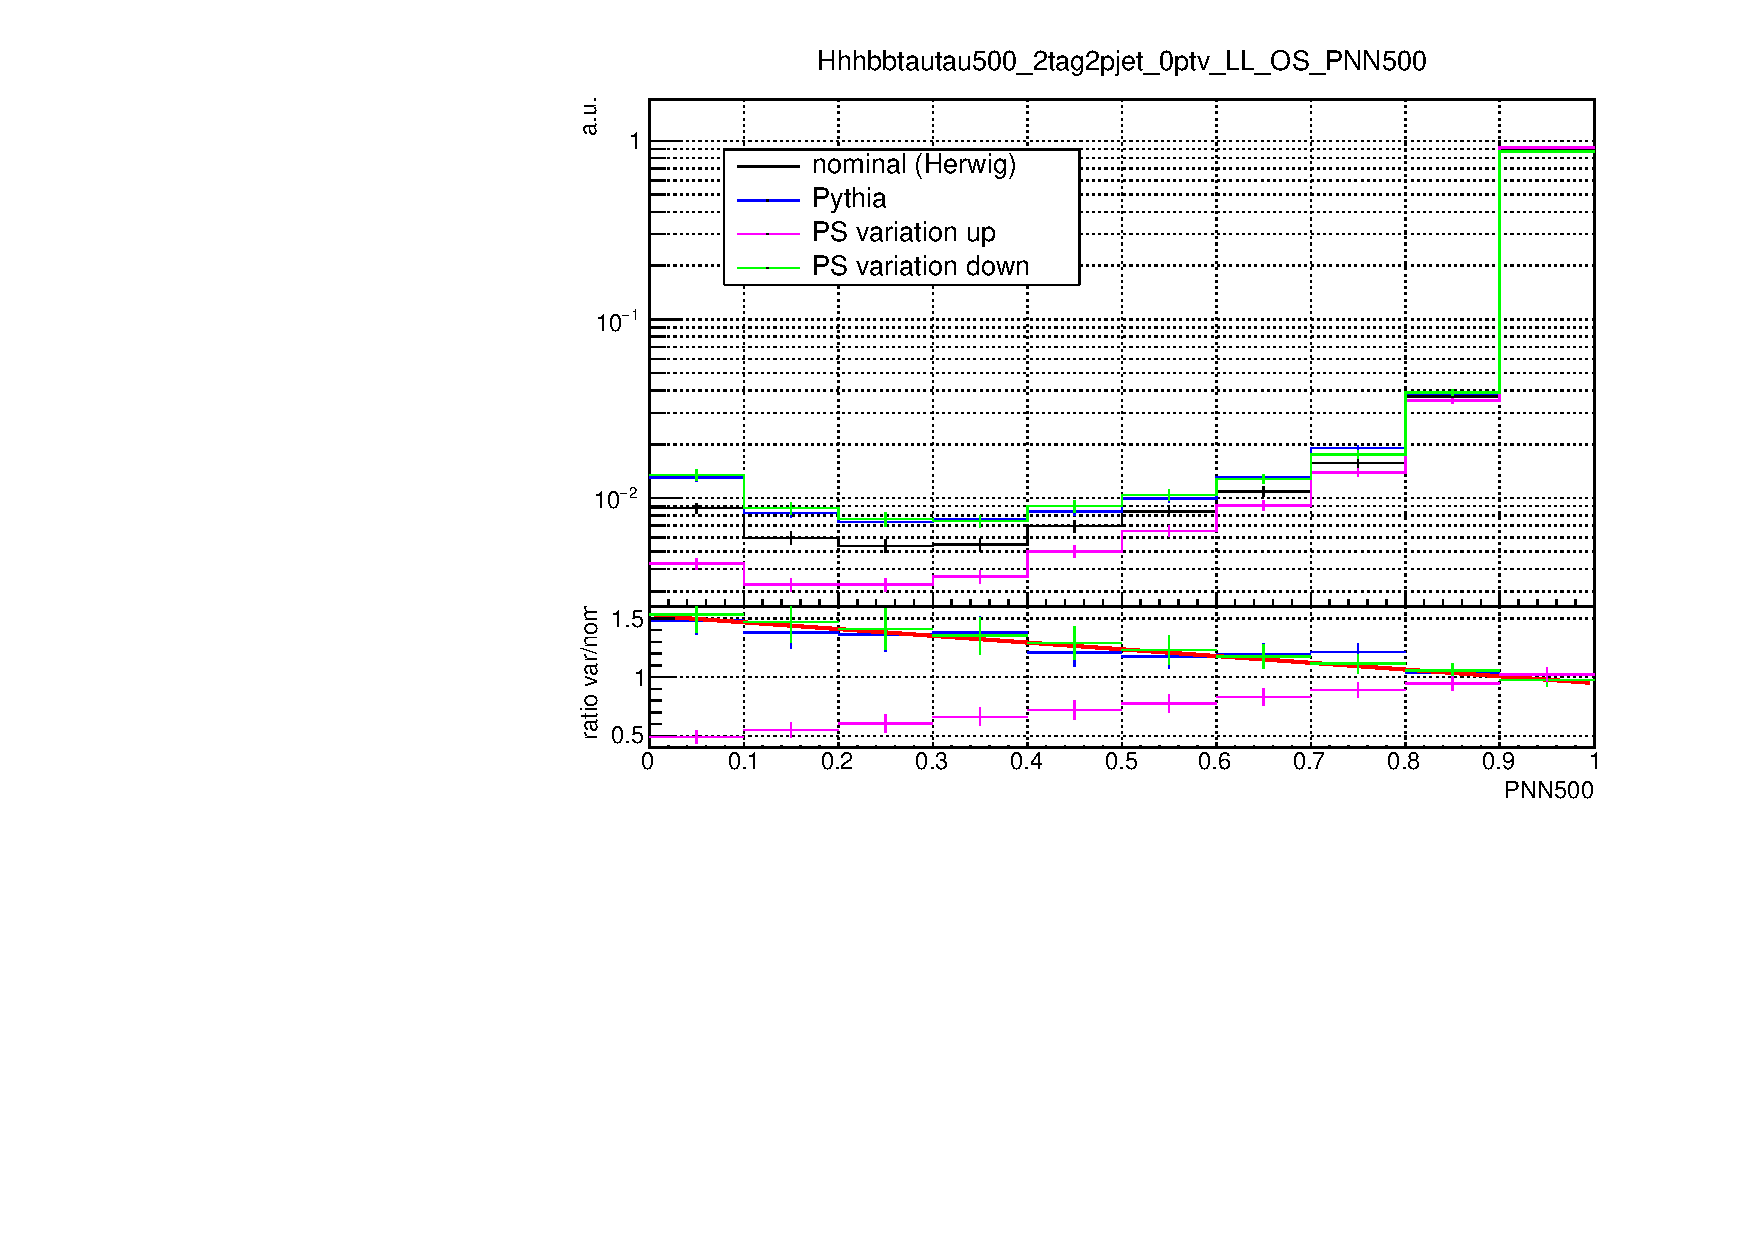
\includegraphics[width=.49\textwidth]{figures/systs/HadHad_Signal_500_PNN_SystsApplied_Fit_log.pdf}
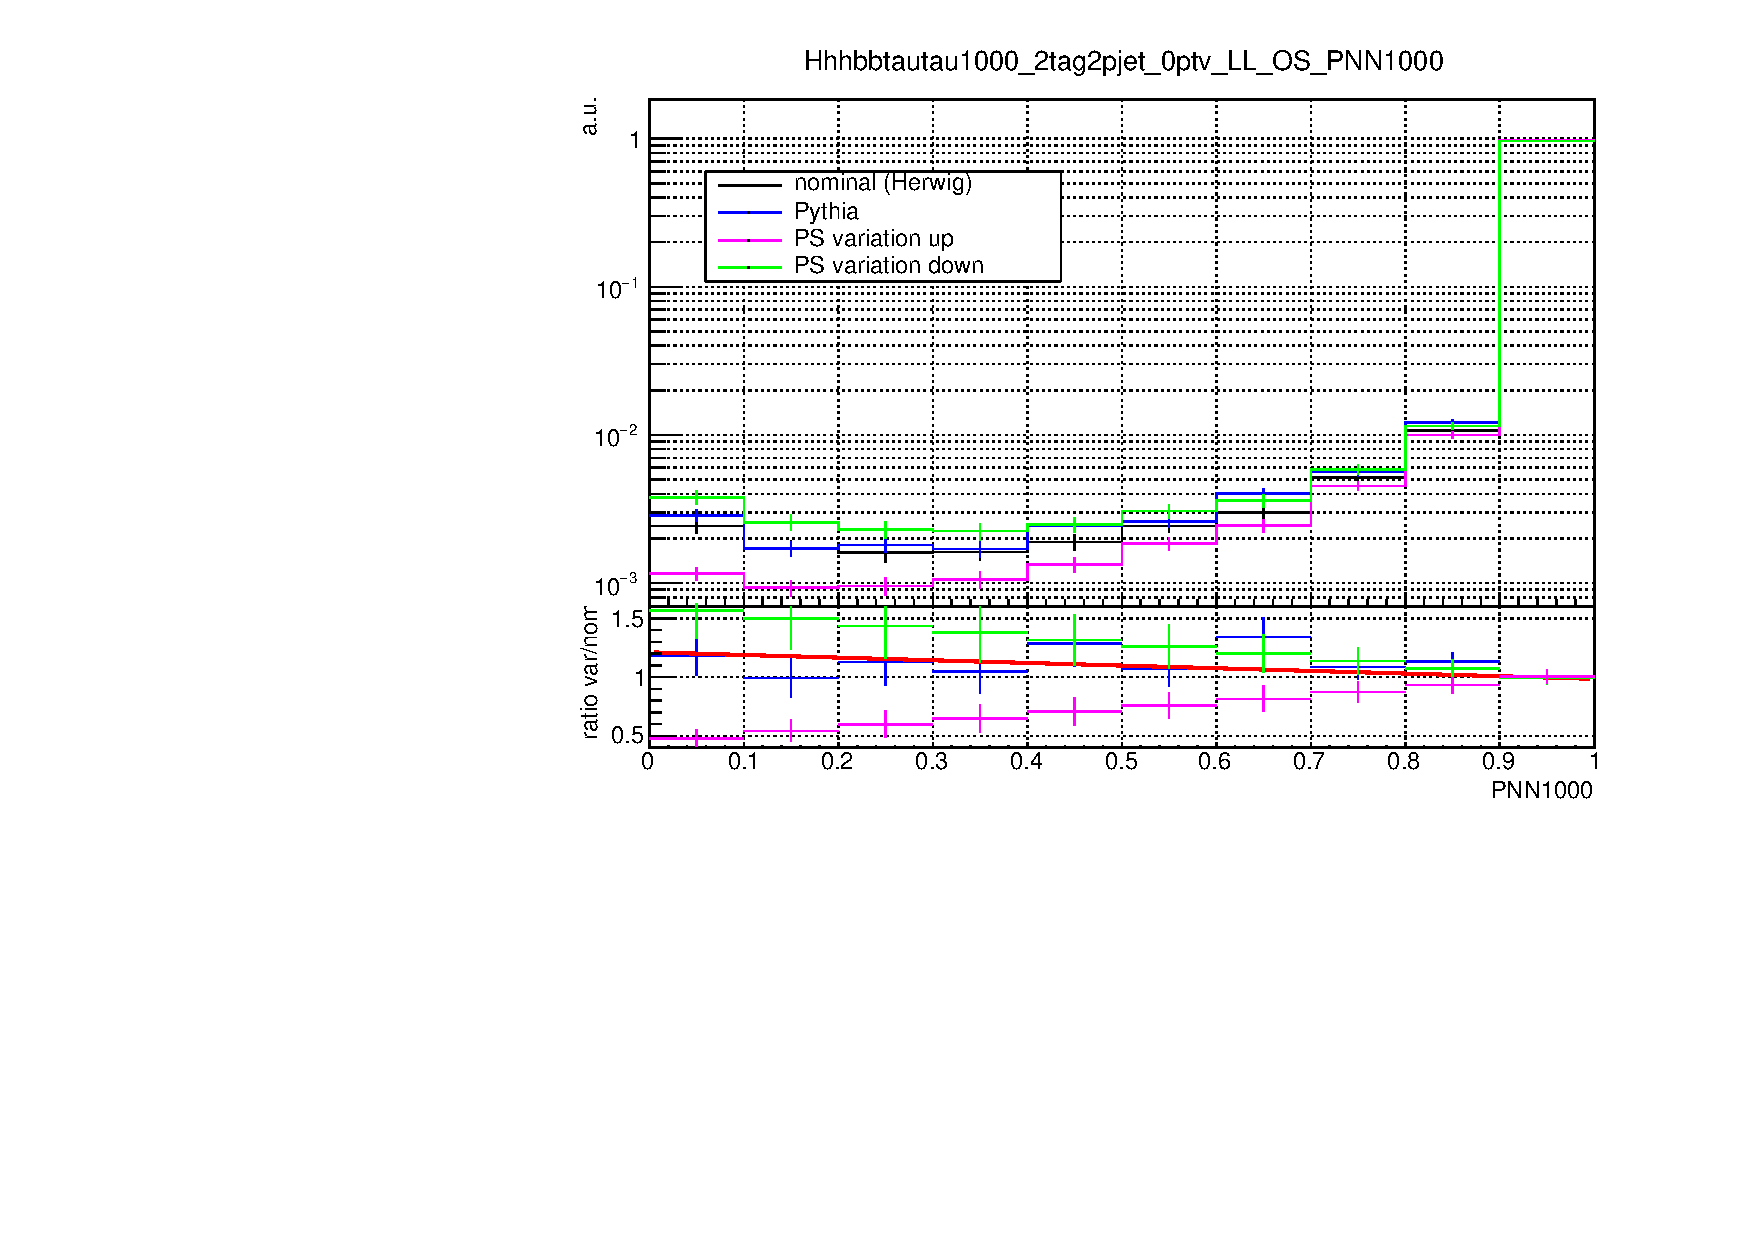
\includegraphics[width=.49\textwidth]{figures/systs/HadHad_Signal_1000_PNN_SystsApplied_Fit_log.pdf}
\caption{Comparison of the di-Higgs $bb\tau_{had}\tau_{had}$ signal PNN distributions obtained from the nominal (black) and alternative (blue) signal samples for the PS variations for the  $m_X= 500$ GeV (left) and the $m_X=1000$ GeV (right) mass points. A linear fit to the ratio of the two distributions is performed and shown in the lower panel of the figures (red line). The variations obtained from the linear function obtained from the $m_X= 500$ GeV fit are also shown in the figures (green and magenta).}
\label{fig:HadHadSignalSysts}
\end{figure}

In the $bb\tau_{lep}\tau_{had}$ channel the overall parton shower acceptance uncertainty on the normalisation is found to be 6\% for $m_X= 500$ GeV and 3\% for  $m_X=1000$ GeV in the SLT SR and 4\% for $m_X= 500$ GeV and 7\% for  $m_X=1000$ GeV in the LTT SR. Thus, a conservative 6\% uncertainty is applied on the normalisation for all mass points in the SLT SR and a conservative 7\% uncertainty is applied on the normalisation for all mass points in the LTT SR.

After taking out the normalisation effect, the acceptance uncertainty on the shape of the PNN distribution is evaluated. Figure~\ref{fig:LepHadSLTSignalSysts} and \ref{fig:LepHadLTTSignalSysts} show the comparisons of the PNN distributions obtained from the nominal (black) and alternative (blue) signal samples for the  $m_X= 500$ GeV and the $m_X=1000$ GeV mass points for the SLT and LTT SRs respectively. A linear fit to the ratio of the two distributions is performed to parameterise the shape variation as a function of the PNN score and shown in the lower panel of the figures (red line). The linear function in the PNN score obtained from the fit performed at $m_X= 500$ GeV has the largest slope so this function is used to obtain the templates for the variations for all mass points. 

The function used in the SLT SR is:

\begin{itemize}
\item Down variation = 1.82 - 0.95 * PNN Score.
\item Up variation = 0.18 + 0.95 * PNN Score;
\end{itemize}

The function used in the LTT SR is:

\begin{itemize}
\item Down variation = 1.84 - 1.01 * PNN Score;
\item Up variation = 0.16 + 1.01 * PNN Score.
\end{itemize}

The variations obtained from this linear function in the PNN score are also shown in the figures (green and magenta) showing that this variation covers the variation given by the alternative samples for the two available mass points in both SRs.

\begin{figure}
\centering
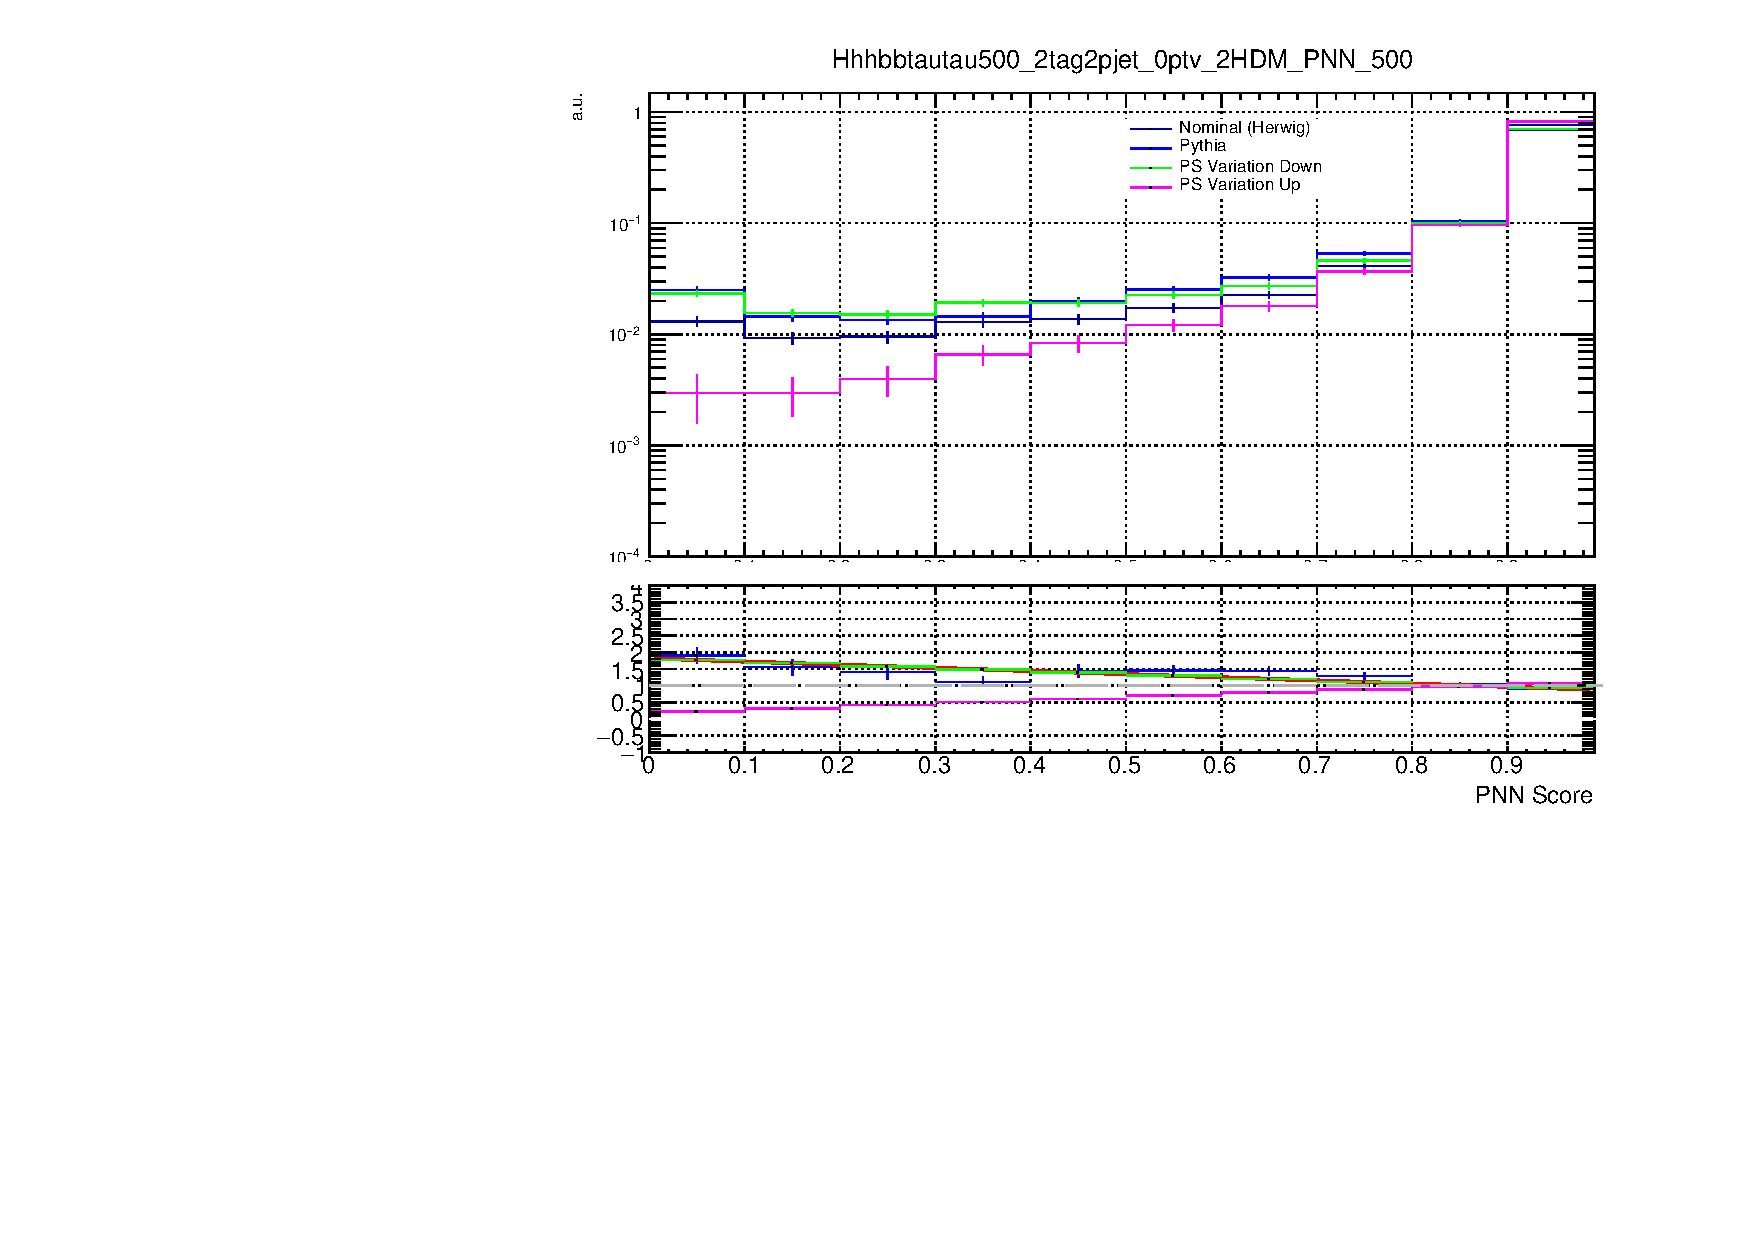
\includegraphics[width=.49\textwidth]{figures/systs/LepHad_Signal_SLT_500_psSysts_PNN_Fit_Logy.pdf}
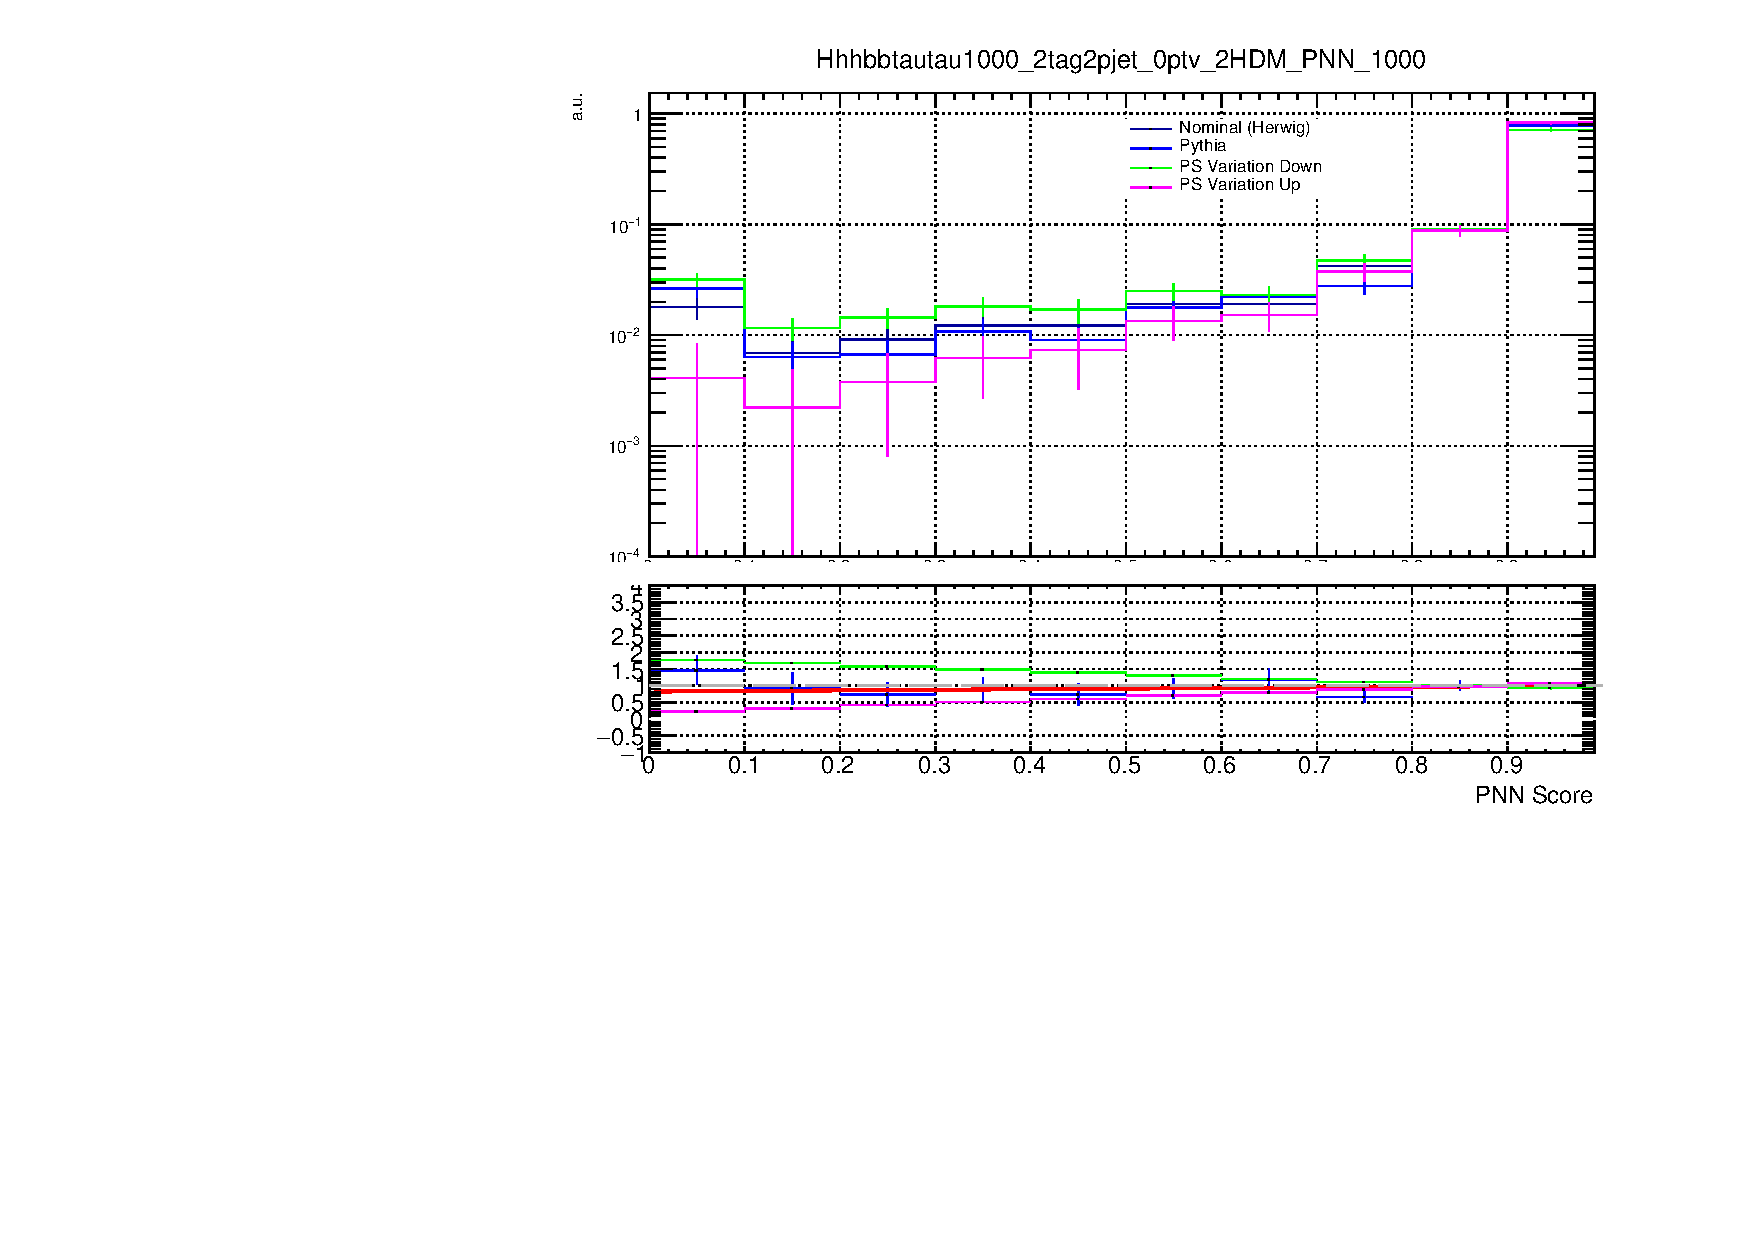
\includegraphics[width=.49\textwidth]{figures/systs/LepHad_Signal_SLT_1000_psSysts_PNN_Fit_Logy.pdf}
\caption{Comparison of the di-Higgs $bb\tau_{lep}\tau_{had}$ SLT signal PNN distributions obtained from the nominal (black) and alternative (blue) signal samples for the PS variations for the  $m_X= 500$ GeV (left) and the $m_X=1000$ GeV (right) mass points. A linear fit to the ratio of the two distributions is performed and shown in the lower panel of the figures (red line). The variations obtained from the linear function obtained from the $m_X= 500$ GeV fit are also shown in the figures (green and magenta).}
\label{fig:LepHadSLTSignalSysts}
\end{figure}

\begin{figure}
\centering
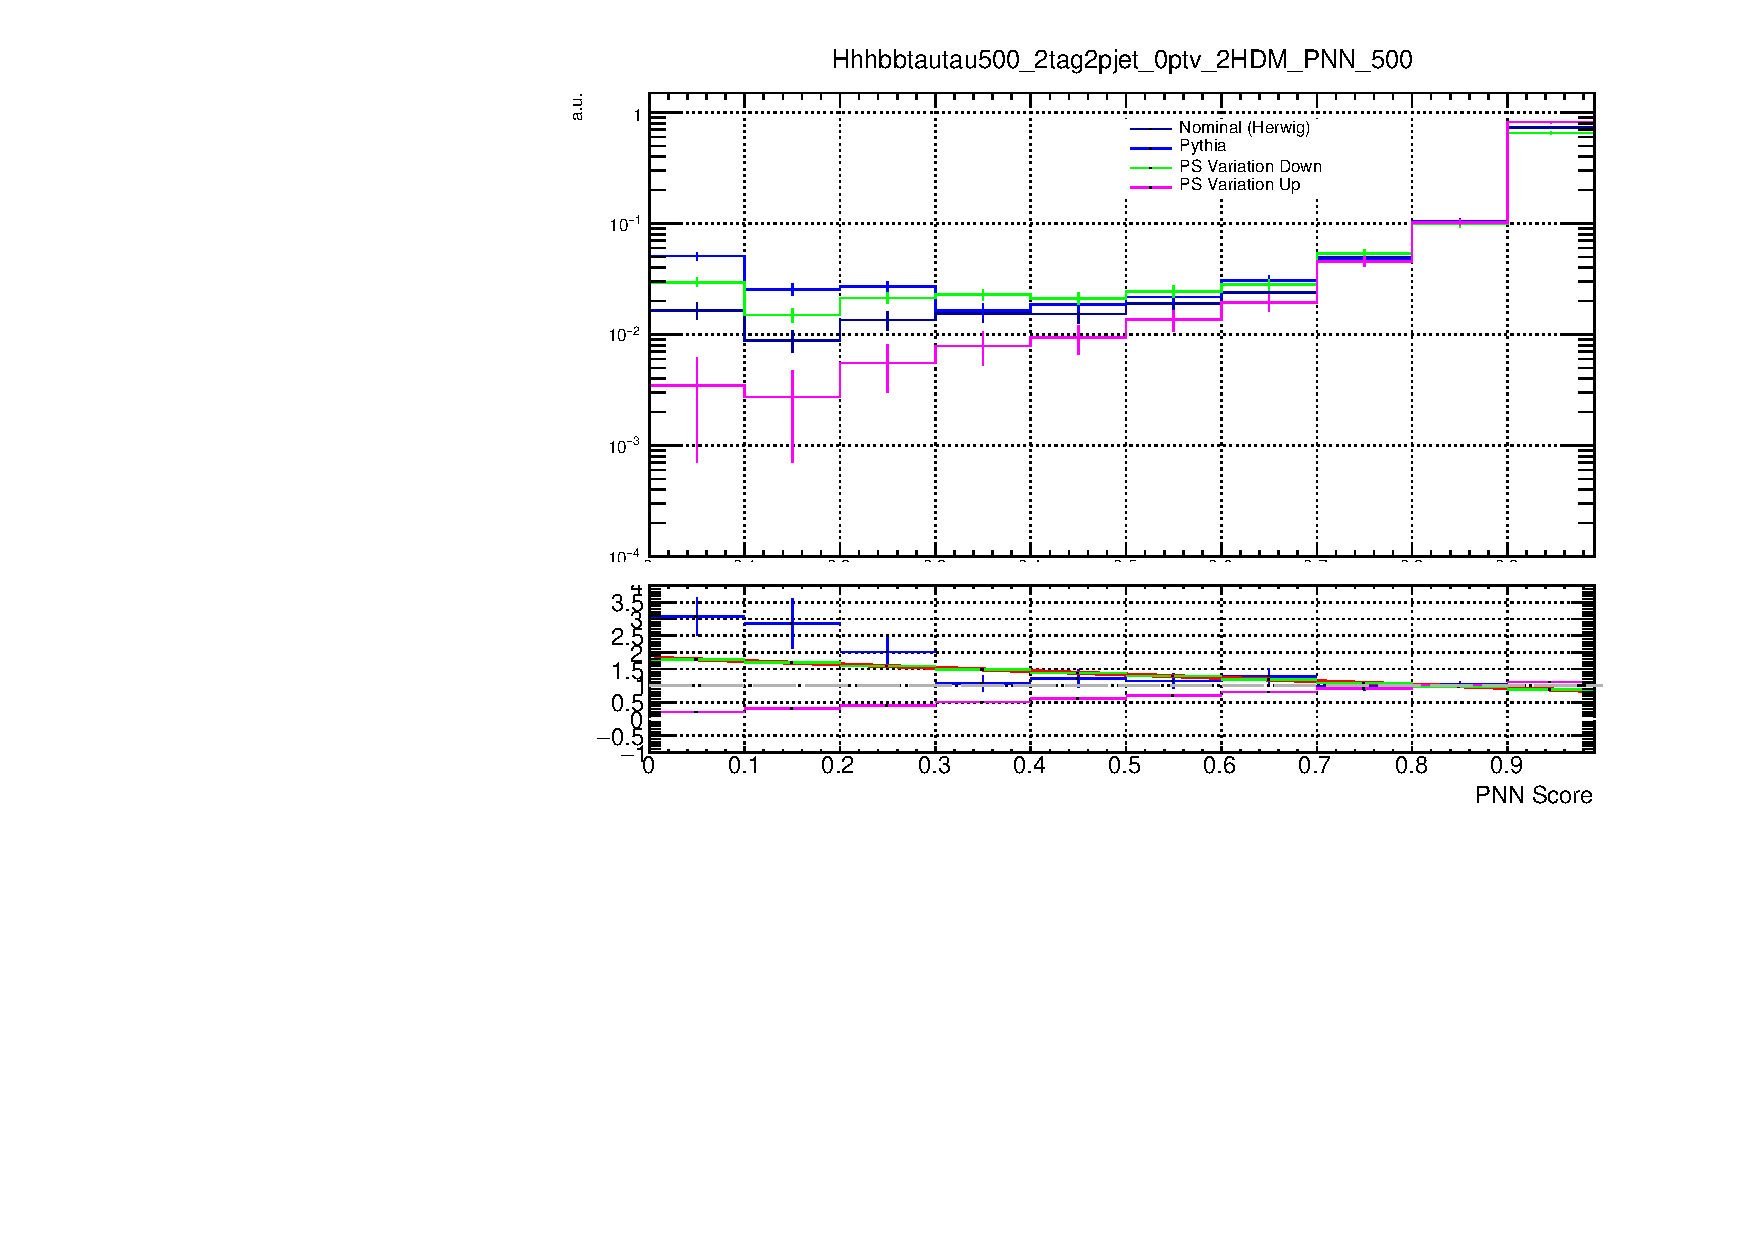
\includegraphics[width=.49\textwidth]{figures/systs/LepHad_Signal_LTT_500_psSysts_PNN_Fit_Logy.pdf}
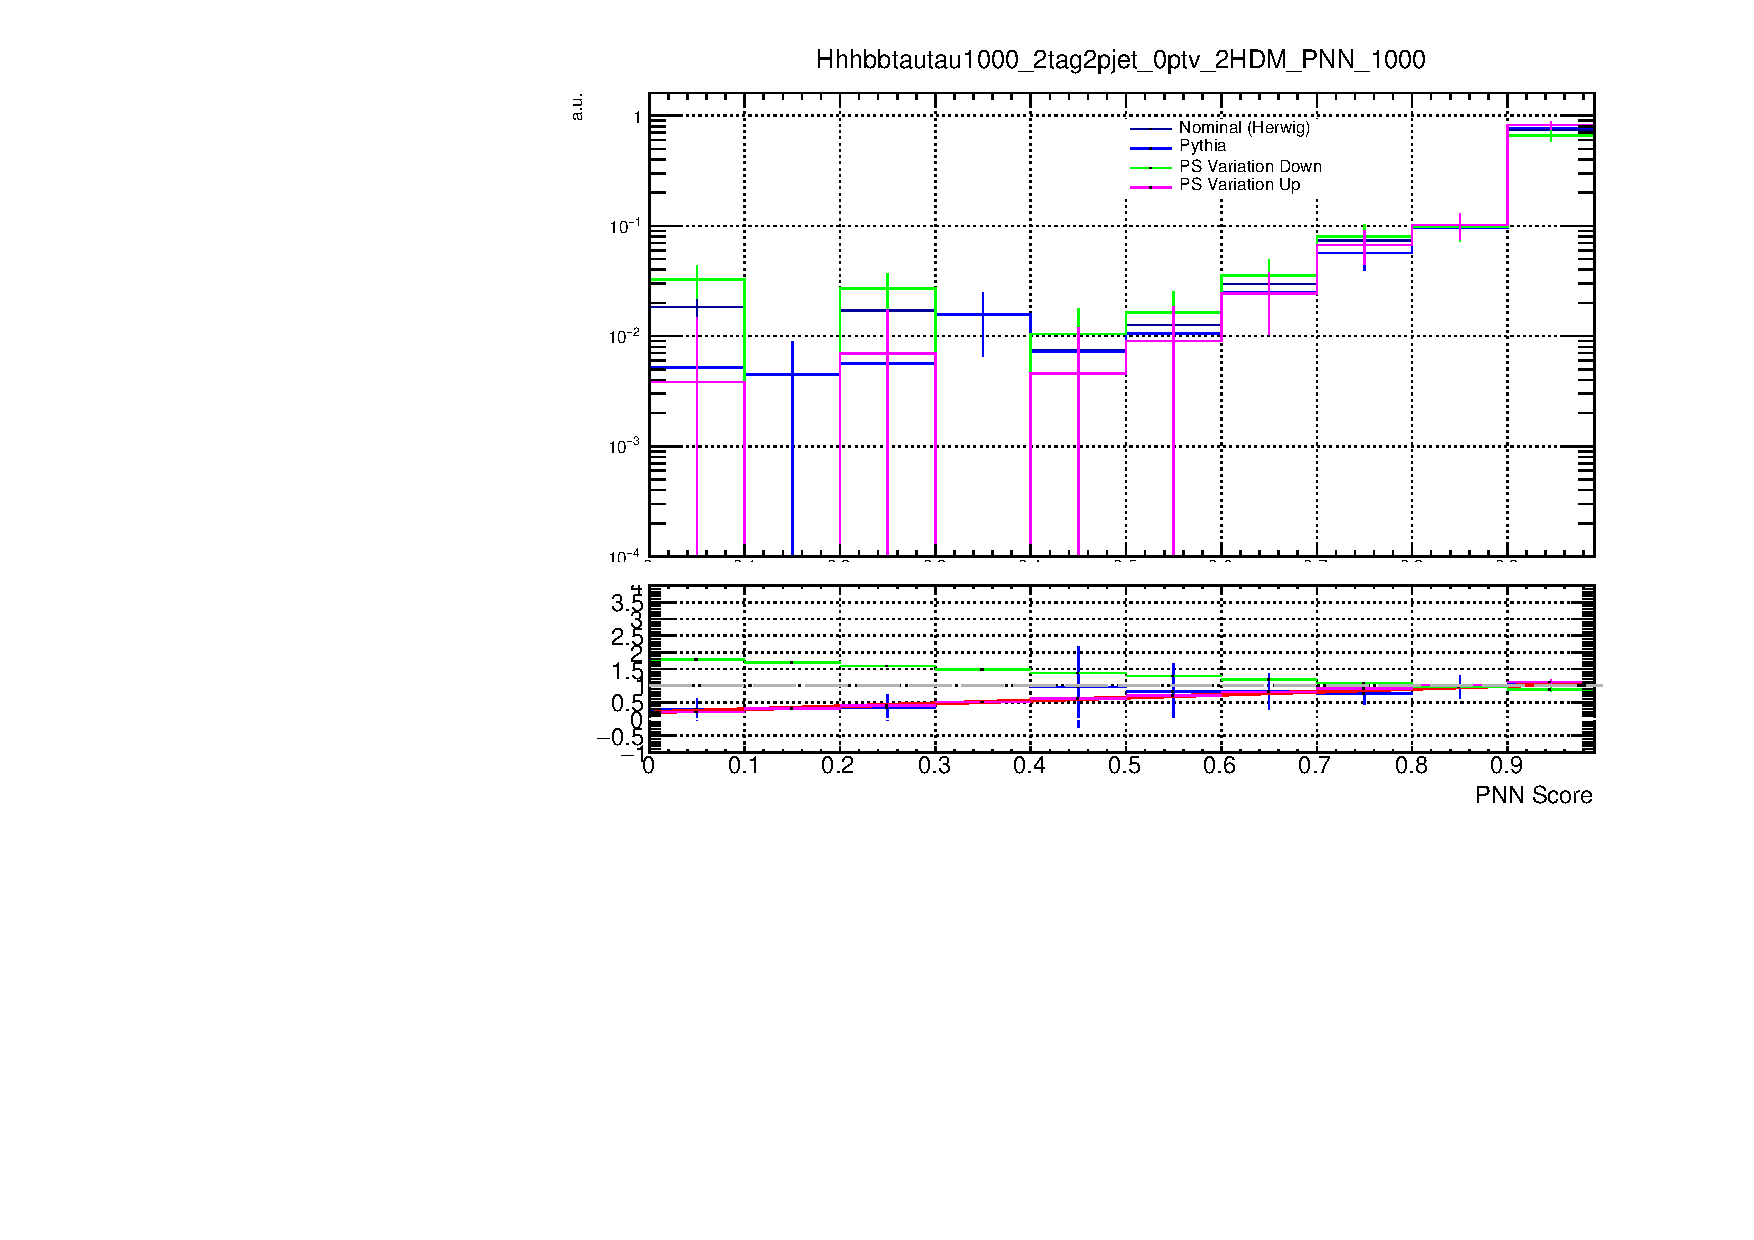
\includegraphics[width=.49\textwidth]{figures/systs/LepHad_Signal_LTT_1000_psSysts_PNN_Fit_Logy.pdf}
\caption{Comparison of the di-Higgs $bb\tau_{lep}\tau_{had}$ LTT signal PNN distributions obtained from the nominal (black) and alternative (blue) signal samples for the PS variations for the  $m_X= 500$ GeV (left) and the $m_X=1000$ GeV (right) mass points. A linear fit to the ratio of the two distributions is performed and shown in the lower panel of the figures (red line). The variations obtained from the linear function obtained from the $m_X= 500$ GeV fit are also shown in the figures (green and magenta).}
\label{fig:LepHadLTTSignalSysts}
\end{figure}

% PDFs and Scales below here

Scale, PDF and $\alpha_s$ uncertainties on signal are expected to be negligible compared to the parton shower uncertainties as it was found in the previous analysis and also in other di-Higgs channels (less than 1\%). They are checked using truth-level samples produced storing alternative weights for these settings. The on-the-fly MadGraphControl framework is used to generate LHE files including alrernative weights. Samples are produced for $m_X=500$ GeV and $m_X=1000$ GeV with 10000 events each. The generated truth-level samples are converted to TRUTH3 derivations and a truth-level analysis is implemented in order to mimic the selection of the analysis and select the same phase-space to evaluate these acceptance uncertainties.

For PDF and $\alpha_s$ variations, the NNPDF30\_ nlo\_s\_ 0118 uncertainty sets, consisting of 100 eigenvectors parameterising the uncertainties for all the PDFs and 1 parameter for the $\alpha_s$ variations, are used and are compared to the nominal NNPDF30\_ nlo\_s\_ 0118 to evaluate the size of the variations (as recommended by the Physics Modelling Group even if the nominal PDF used in the nominal sample is the NNPDF23\_ lo\_ as\_ 0130\_ qed set). These variations are combined following the recommendations~\cite{Butterworth:2015oua}, consisting in evaluating the PDF uncertainty $\delta_{PDF}$ by calculating the square root of the sum in quadrature of the 30 variations, evaluating the $\alpha_s$ uncertainty by taking the half difference between the same PDF set with two different $\alpha_s$ values, and then adding in quadrature the two contributions of $\delta_{PDF}$ and $\alpha_s$ uncertainties to obtain the total uncertainty. 

As alternative weights are available also for the alternative PDF sets MMHT2014nlo68clas118 and the CT14nlo these are also checked. Alternative weights are available also for the PDF4LHC\_ NLO\_ 30 uncertainty sets which consist of 30 eigenvectors for all the PDFs and 1 parameter for the $\alpha_s$ variations and these are also checked as a cross-check. 

Scale uncertainties are evaluated using the 7-point scale variations of the renormalisation ($\mu_R$) and the factorisation scale ($\mu_F$) which are combined by taking an envelope of all of the variations (as recommended by the Physics Modelling group). 

All acceptance uncertainties on the signal normalisation obtained in the different signal regions are shown in Table~\ref{sec:systs:tab:systematics_HHSignal_AcceptanceNumbers}.  

The PDF+$\alpha_s$ uncertainties obtained from the NNPDF30\_ nlo\_s\_ 0118 uncertainty set are found to be negligible compared to the Parton Shower uncertainties and the uncertainties obtained from PDF4LHC\_ NLO\_ 30 uncertainty set and from the two alternative PDF sets are well within the NNPDF30\_ nlo\_s\_ 0118 variations. The effect of PDF+$\alpha_s$ uncertainties on the shapes of the PNN input variables is also checked and found to be negligible as shown in Appendix~\ref{subsec:appendix_systs_signalsysts}. Thus, the PDF+$\alpha_s$ uncertainties on signal are neglected in the analysis. 

The scale uncertainties are also found to be negligible compared to the Parton Shower uncertainties and their effect on the shapes of the PNN input variables is also is also checked and found to be negligible as shown in Appendix~\ref{subsec:appendix_systs_signalsysts}. Thus, the scale uncertainties on signal are neglected in the analysis. 

As the resonant samples are generated with AF2 for masses up to 1 TeV (from \SI{1.1}{\TeV}
full simulation is used), the difference between the AF2 samples and
the full simulation samples is checked.  

In the \lephad channel, the
check is done using the 400 GeV mass point sample of 2017 and 2018
(mc16d, mc16e) MC.  The difference is less than 1\% in the SLT channel
and 2.9\% in the LTT channel, and there is no obvious shape
difference between the two types of simulation, as shown in
Figure~\ref{fig:Lephad_resonant_AF2_VS_FS}. 
As discussed in the following paragraph, it was found that the larger difference in acceptance times efficiency in 
LTT is originating from the \tauhad 
triggers for which no dedicated recommendations for AF2 exist.
Therefore a 3\% acceptance uncertainty is assigned to LTT of all signal
samples simulated with AF2 (up to 1TeV mass point).

\begin{figure}
  \centering
  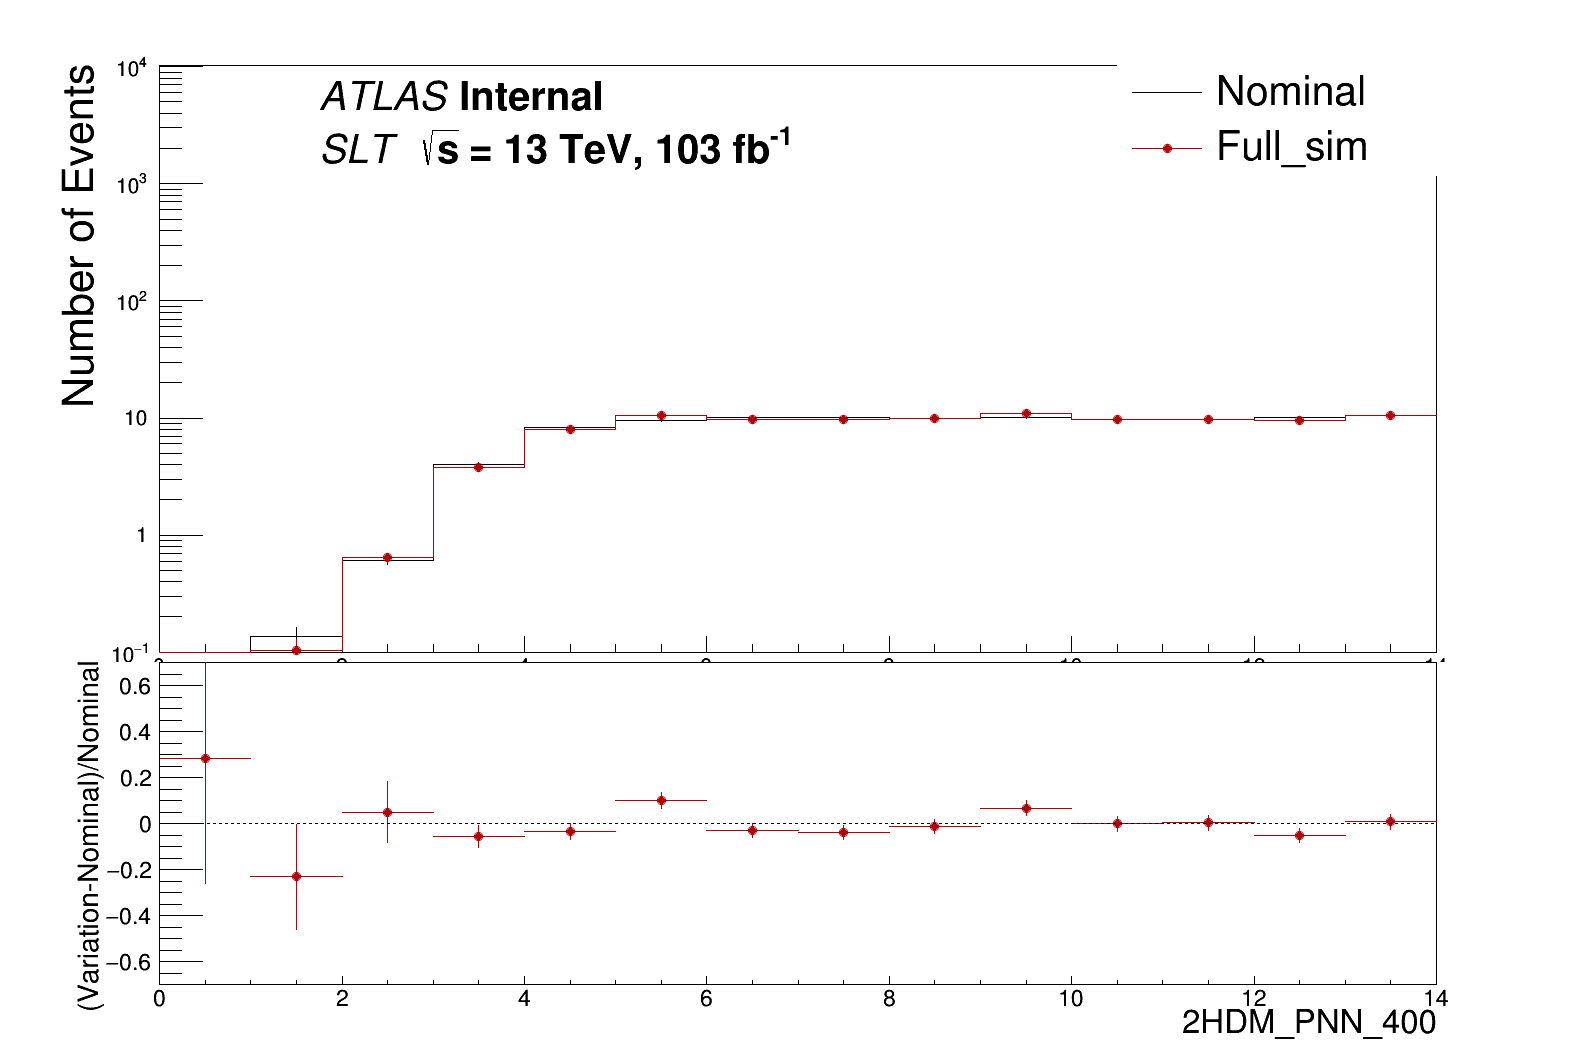
\includegraphics[width=.49\textwidth]{figures/lephad_modelling_systs/SLT/signal_AF2_check/limit_binning_2HDM_PNN_400_Norm.png}
  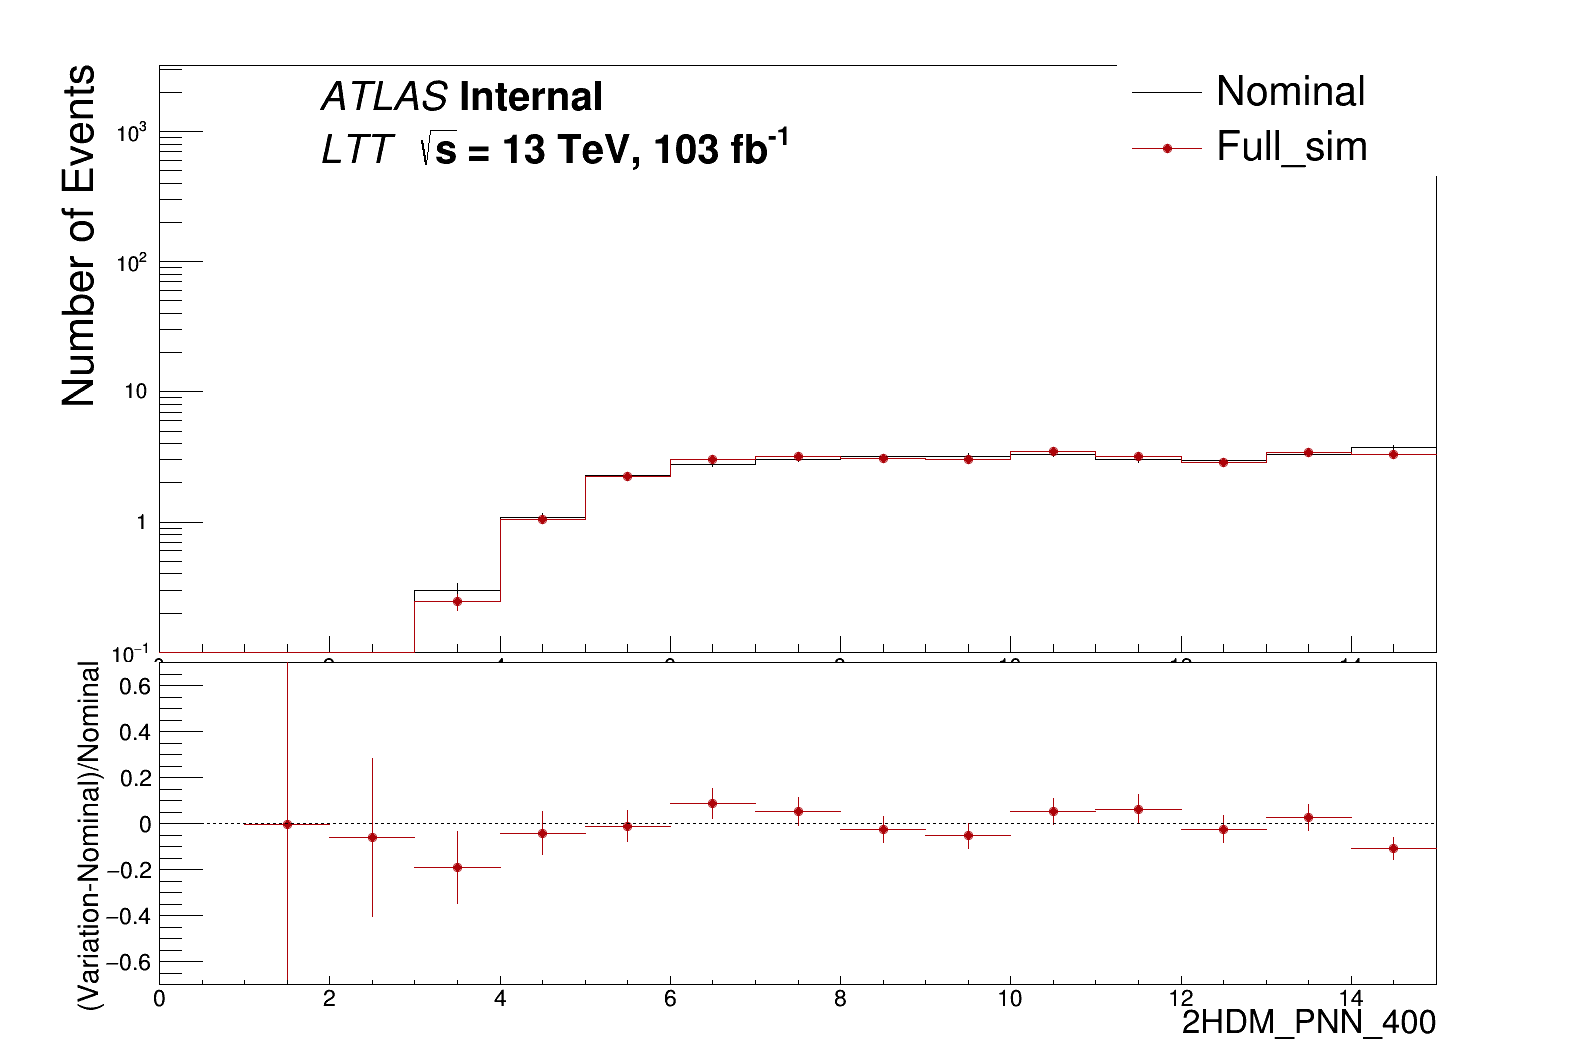
\includegraphics[width=.49\textwidth]{figures/lephad_modelling_systs/LTT/signal_AF2_check/limit_binning_2HDM_PNN_400_Norm.png}
  \caption{Comparison of the di-Higgs \lephad signal PNN distributions obtained from the nominal (AF2)
    and alternative (full simulation) signal samples for the  $m_X= 400$ GeV for the
    SLT (left) and the LTT (right) channel. The binning is the same as the final fit binning.
  }
  \label{fig:Lephad_resonant_AF2_VS_FS}
\end{figure}

In the \hadhad-channel the acceptance of the resonant signal is
compared between full- and fast-simulation using the \SI{400}{\GeV}
$\text{X} \to \text{HH}$ simulated sample using MC16A
only\footnote{The primary AODs for the full-simulation MC16D and MC16E
  samples were unfortunately deleted due to the obsolesence procedure
  and thus were not available for this study.}. A statistically
significant deviation of more than three standard deviations is
observed in the overall acceptance times efficiency of the \hadhad SR selection. The
fast-simulation tends to overestimate the signal yield by 6.5~\% in
the \hadhad SR. Comparing the cutflows between fast- and
full-simulation (c.f.\ \Cref{tab:cutflow_fullsim_fastsim_hadhad}), it
was determined that this discrepancy is originating from the \tauhad
triggers for which no dedicated recommendations for AF2 exist. The
distribution of the final discriminant (PNN400) was compared for both
samples which showed no discernable impact on the shape of the
distribution. Additionally, the impact was compared between the STT
and DTT trigger-channels showing equal impact in both. Therefore, a
6.5~\% normalization uncertainty is assigned to all signal samples
simulated using AF2 (i.e.\ up to the 1 TeV mass
point). 

\begin{table}
\centering
\small
\begin{tabular}{|c|c|c|c|c|}
\hline
Process X, GeV& HadHad & LepHad SLT  & LepHad LTT & Description\\
\hline
$m_{X}= 400$ & 0.065 &  <0.01 & 0.029 & AF2\\
$m_{X}= 500$ & 0.093 &  0.06 & 0.05 & Parton Shower\\
$m_{X}= 500$ & 0.001 &  0.0033 & 0.023 & PDF+$\alpha_s$ from NNPDF30\_ nlo\_s\_ 0118\\
$m_{X}= 500$ & 0.00013 &   0.00031 &  0.00051 & Alt. PDF from MMHT2014nlo68clas118\\ %UPDATE HADHAD
$m_{X}= 500$ & 0.00029 &  0.000063 &  0.00046 & Alt. PDF from CT14nlo\\ 
$m_{X}= 500$ & 0.00055 &  0.00078 &  0.0020 & PDF+$\alpha_s$ from PDF4LHC\\ 
$m_{X}= 500$ & 0.00015 &  0.00048 &  0.0012 & Scales \\
$m_{X}= 1000$ & 0.062 &  0.03 &  0.07 & Parton shower\\
$m_{X}= 1000$ & 0.00077 &  0.0094 &  0.029 & PDF+$\alpha_s$ from NNPDF30\_ nlo\_s\_ 0118\\
$m_{X}= 1000$ & 0.00007 &  0.00034 &   0.0009 & Alt. PDF from MMHT2014nlo68clas118\\ %UPDATE HADHAD
$m_{X}= 1000$ & 0.00008 &   0.00029 &  0.0024 & Alt. PDF from CT14nlo\\ 
$m_{X}= 1000$ & 0.00051 &   0.0013 &  0.0069 & PDF+$\alpha_s$ from PDF4LHC\\ 
$m_{X}= 1000$ & 0.00015 &   0.00067 &  0.0019  & Scales \\
\hline
\end{tabular}
\caption{List and relative size of the ggF HH resonant signal acceptance uncertainties in the individual signal regions.}
\label{sec:systs:tab:systematics_HHSignal_AcceptanceNumbers}
\end{table}


%PDF+alphas HadHad
%n the di-Higgs $bb\tau_{had}\tau_{had}$ channel the overall PDF+$\alpha_s$ acceptance uncertainty on the normalisation is found to be 0.10\% for $m_X= 500$ GeV and 0.077\% for  $m_X=1000$ GeV using the NNPDF30\_ nlo\_s\_ 0118 uncertainty sets. 
%As alternative weights are available also for the alternative PDF sets MMHT2014nlo68clas118 and the CT14nlo these are also checked. The largest variation comes from the CT14nlo PDF set and it is of 0.029\% for $m_X= 500$ GeV and 0.008\% for $m_X= 1000$ GeV, so well within the NNPDF30\_ nlo\_s\_ 0118 variations and thus neglected.  
%Alternative weights are available also for the PDF4LHC\_ NLO\_ 30 uncertainty sets which consist of 30 eigenvectors for all the PDFs and 1 parameter for the $\alpha_s$ variations and these are also checked as a cross-check. The PDF+$\alpha_s$ acceptance uncertainty on the normalisation is found to be 0.0055\% for $m_X= 500$ GeV and 0.051\% for  $m_X=1000$ GeV using the PDF4LHC\_ NLO\_ 30 uncertainty sets (smaller than the uncertainties from the NNPDF30\_ nlo\_s\_ 0118 uncertainty sets).
%The effect of PDF+$\alpha_s$ uncertainties on the shapes of the PNN input variables is also checked and found to be negligible as shown in Appendix~\ref{subsec:appendix_systs_signalsysts}.
%Thus, the PDF+$\alpha_s$ uncertainties on signal are neglected in the analysis. 

%Scale HadHad
%In the di-Higgs $bb\tau_{had}\tau_{had}$ channel the scale acceptance uncertainty on the normalisation is found to be 0.015\% for both $m_X= 500$ GeV and  $m_X=1000$ GeV. The effect of the scale uncertainties on the shapes of the PNN input variables is also checked and found to be negligible as shown in Appendix~\ref{subsec:appendix_systs_signalsysts}.
%Thus, the scale uncertainties on signal are neglected in the analysis.

\subsubsection{Non-resonant signal}

\paragraph{ggF non-resonant}

Acceptance uncertainties on the non-resonant production of di-Higgs via ggF are derived using the recommendations from PMG.

The parton shower uncertainties are estimated by comparing the nominal samples showered with Pythia8 to alternative samples showered with Herwig7. The alternative samples used for the parton shower uncertainties are reported in Table~\ref{sec:systs:tab:systematics_NonRessignalsamples}.


\begin{table}
\centering
\begin{tabular}{|c|c|}
\hline
DSID & Name\\
\hline
600023 & PhH7EG\_PDF4LHC15\_HHbbtautauHadHad\_cHHH01d0\\
600024 & PhH7EG\_PDF4LHC15\_HHbbtautauHadHad\_cHHH10d0\\
600029 & PhH7EG\_PDF4LHC15\_HHbbtautauLepHad\_cHHH01d0\\
600030 & PhH7EG\_PDF4LHC15\_HHbbtautauLepHad\_cHHH10d0\\
\hline
\end{tabular}
\caption{List of alternative di-Higgs non-resonant signal samples for PS uncertainties.
}
\label{sec:systs:tab:systematics_NonRessignalsamples}
\end{table}


In the \hadhad channel the overall parton shower acceptance uncertainty on the normalisation is found to be 4.3\% and 5.1\% for the SM non-resonant signal and for the $\kappa_\lambda=10$ non-resonant signal, respectively.  In the \lephad channel it is found to be for the SM signal 7.6\% in SLT and 7.5\% in LTT.

Uncertainties from PDF, $\alpha_s$ and scales are evaluated using alternative weights available in the nominal samples.

PDF and $\alpha_s$ uncertainties are evaluated using the alternative weights for the PDF4LHC\_ NLO\_ 30 uncertainty sets which consist of 30 eigenvectors for all the PDFs and 1 parameter for the $\alpha_s$ variations. These variations are combined following the recommendations~\cite{Butterworth:2015oua}, consisting in evaluating the PDF uncertainty $\delta_{PDF}$ by calculating the square root of the sum in quadrature of the 30 variations, evaluating the $\alpha_s$ uncertainty by taking the half difference between the same PDF set with two different $\alpha_s$ values, and then adding in quadrature the two contributions of $\delta_{PDF}$ and $\alpha_s$ uncertainties to obtain the total uncertainty. 

In the \hadhad channel PDF+$\alpha_s$ uncertainties are found to be 0.1\% and 0.7\% on the non-resonant SM signal and the non-resonant $\kappa_\lambda$ signal respectively and are thus neglected in the analysis as they are below 1\%. In the \lephad channel they are found to be for the SM signal 0.6\% in SLT and 0.7\% in LTT and are also neglected in the analysis.

Scale uncertainties are evaluated using the 7-point scale variations of the renormalisation ($\mu_R$) and the factorisation scale ($\mu_F$) which are combined by taking an envelope of all of the variations (as recommended by the Physics Modelling group). 

In the \hadhad channel the scale uncertainties are found to be 1.4\% on both the non-resonant SM signal and the non-resonant $\kappa_\lambda$ signal respectively and are included in the analysis.  In the \lephad channel they are found to be for the SM signal 1.2\% in SLT and 1\% in LTT.

After taking out the normalisation effects, shape effects were checked on the MVA score distributions and found to be negligible as reported in Appendix~\ref{subsec:appendix_systs_signalsysts} and therefore are not considered in the analysis.



\begin{table}
\centering
\small
\begin{tabular}{|c|c|c|c|c|}
\hline
Process & HadHad & LepHad SLT & LepHad LTT & Description\\
\hline
SM  & 0.043 &  0.076 & 0.075 & Parton Shower\\
SM & 0.0010 &  0.0061 &  0.0072 & PDF+$\alpha_s$ from PDF4LHC\\ 
SM & 0.014 &  0.012 &  0.010 & Scales \\
$\kappa_\lambda=10$ & 0.051 &  ? & ? & Parton Shower\\
$\kappa_\lambda=10$ & 0.007 &  ? &  ? & PDF+$\alpha_s$ from PDF4LHC\\ 
$\kappa_\lambda=10$ & 0.014 &  ? &  ? & Scales \\
\hline
\end{tabular}
\caption{List and relative size of ggF HH non-resonant signal acceptance uncertainties in the individual signal regions.}
\label{sec:systs:tab:systematics_HHNonResSignal_AcceptanceNumbers}
\end{table}

Cross section uncertainties are also included, with values from \href{https://twiki.cern.ch/twiki/bin/view/LHCPhysics/LHCHWGHH?redirectedfrom=LHCPhysics.LHCHXSWGHH#Latest_recommendations_for_gluon}{\underline{LHCHHWG}} recommendations, shown in Table~\ref{sec:systs:tab:systematics_HHNonResSignal_XSecNumbers}.

\begin{table}
\centering
\small
\begin{tabular}{|c|c|}
\hline
Source & Uncertainty\\
\hline
%Scale & -0.05, +0.022\\
%PDF & 0.021\\
%$\alpha_s$ & 0.021\\
%Mtop approx.  & 0.026\\
Combined Scale+MTop & -0.23, +0.06\\
Combined PDF+$alpha_s$ & -0.03, +0.03\\
\hline
\end{tabular}
\caption{List and relative size of ggF HH non-resonant SM signal cross section uncertainties.}
\label{sec:systs:tab:systematics_HHNonResSignal_XSecNumbers}
\end{table}


\paragraph{VBF non-resonant}

Acceptance uncertainties on the non-resonant production of di-Higgs
via VBF are derived using the recommendations from PMG. 

The acceptance uncertainties from missing higher orders are derived by
varying the factorization $\mu_\text{F}$ and renormalization scale
$\mu_\text{R}$ independently and coherently resulting in 7 settings
for the scales (including the nominal). 

The effect of these variations
on the normalization of the signal in the \hadhad-channel is
negligible. A small (less than 2 \%) shape-impact on the final
discriminant in the \hadhad-channel is observed
in~\Cref{fig:vbf_uncertainties_scale_pdf}. This shape is directly
propagated using the internal weights to the fit. 
The signal acceptance uncertainty due to scale variations is derived as 0.86\% (0.63\%) for the \lephad SLT (LTT) channel.
Corresponding distributions can be found in~\Cref{fig:lephad_vbf_scale_pdf}.


The PDF+\alphas uncertainties are derived using the error set of the
NNPDF30NLO PDF used for the generation of the signal
sample. Additionally, the value of \alphas is varied from 0.118 to
0.119 and 0.117 to evaluate the impact of the choice of \alphas. These
two sources of uncertainties are combined by adding them in
quadrature. 

Both in the \hadhad and \lephad channels, the PDF+\alphas uncertainty shows
no shape impact on the final discriminants
(c.f.~\Cref{fig:vbf_uncertainties_scale_pdf} for the \hadhad and ~\Cref{fig:lephad_vbf_scale_pdf} for the \lephad channels, respectively). The overall norm
uncertainty is well below 1\% therefore a conservative uncertainty of
1\% (max fluctuation observed) is assigned to the non-resonant production of di-Higgs via VBF in
the \hadhad-channel. In the \lephad channel, this uncertainty is calculated as 0.15\% (0.23\%) for the SLT (LTT) channel,
and therefore found negligible.

\begin{figure}[htbp]
  \centering

  \subfloat[]{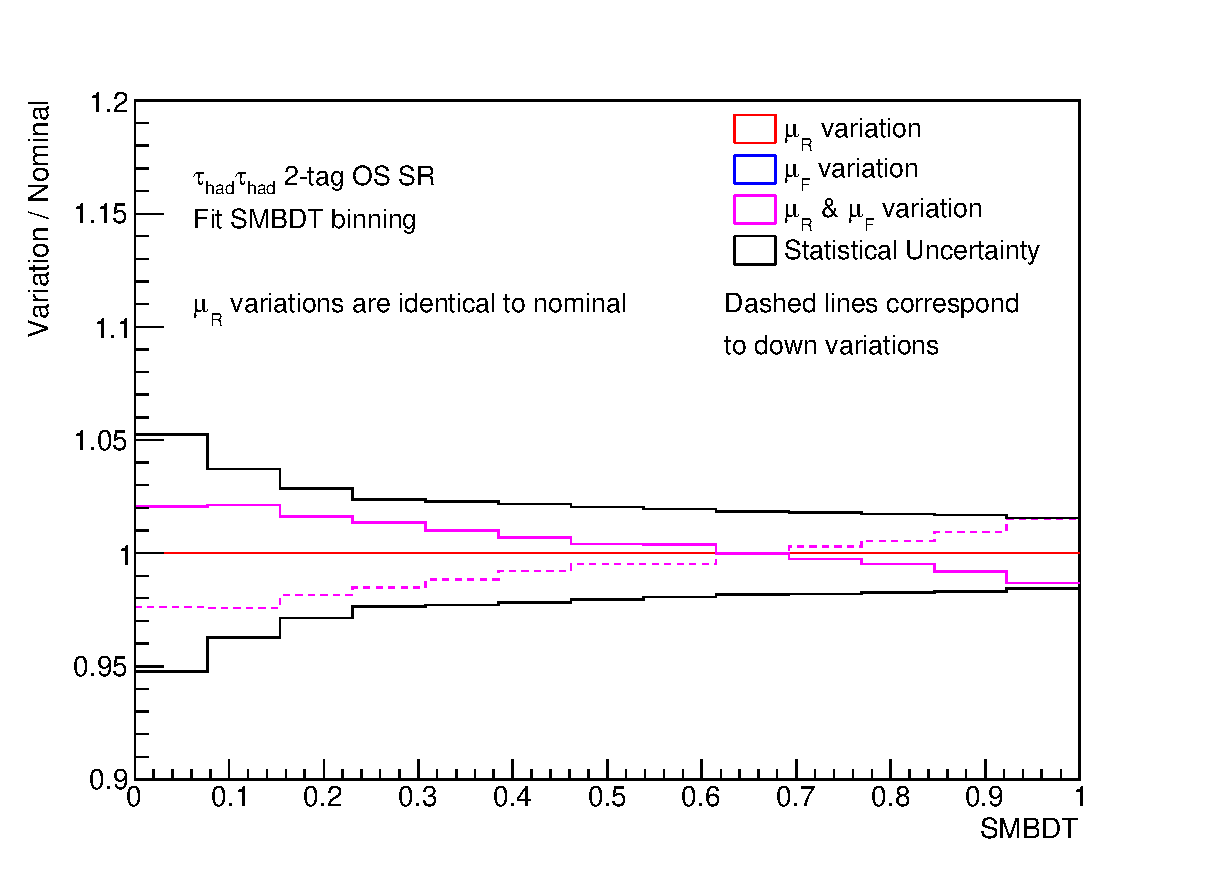
\includegraphics[width=0.5\textwidth]{figures/systs/hadhad_vbf/scale}}%
  \subfloat[]{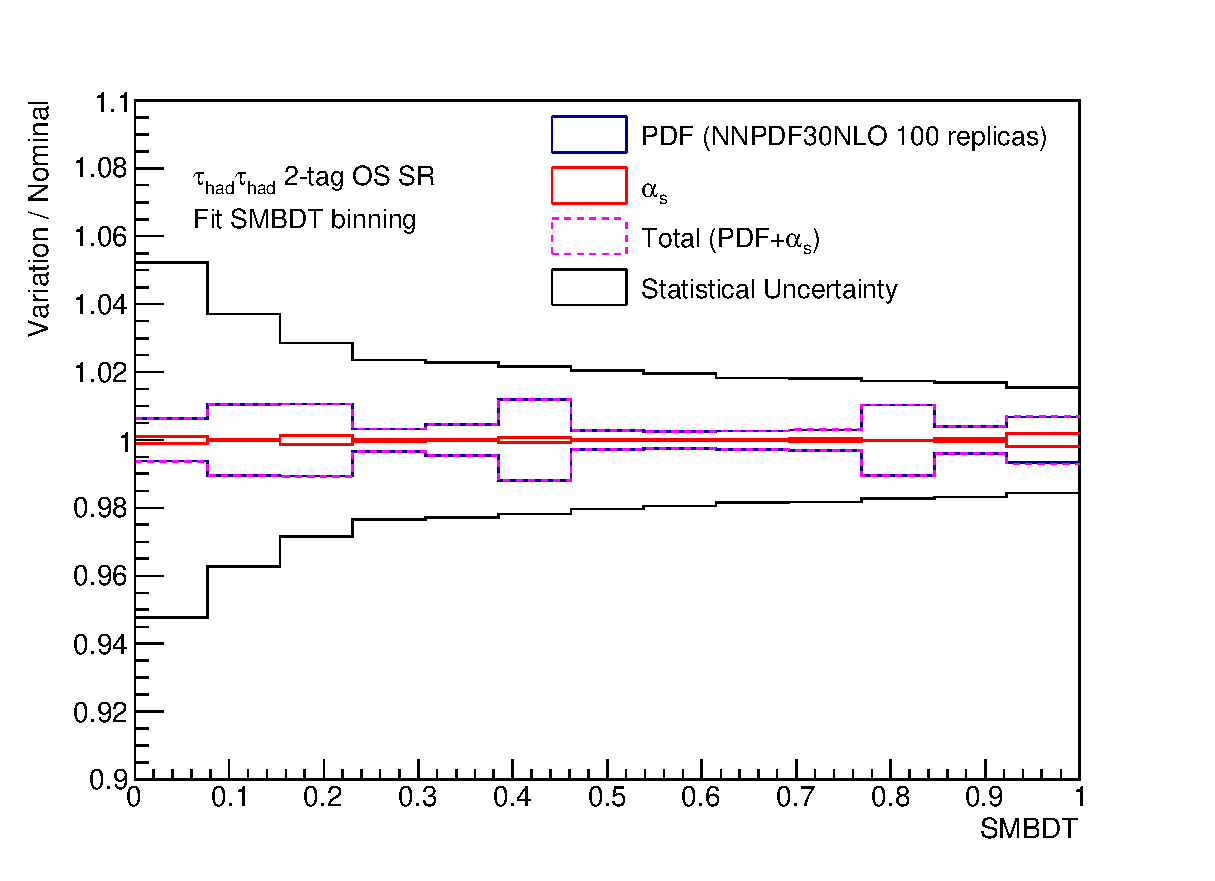
\includegraphics[width=0.5\textwidth]{figures/systs/hadhad_vbf/pdf}}

  \caption{Impact of the 7-point scale variations on the final
    discriminant (SMBDT) in the SR of the \hadhad-channel (a) and the
    PDF+\alphas uncertainties (b). The shape-impact of the
    factorization scale variation is propagated using the internal
    weights to the final discriminant.}
  \label{fig:vbf_uncertainties_scale_pdf}
\end{figure}

Finally, the nominal VBF signal sample showered with Pythia8 is
compared to an alternative sample using Herwig7 for the parton
shower. The alternative PS shows no significant
shape impact on the final discriminants, therefore a 3\% uncertainty
on the normalisation is assigned in the \hadhad channel, whereas a 6.3\% (2.1\%) uncertainty 
is assigned in the SLT (LTT) \lephad channel. The comparison of parton shower
algorithms is shown in~\Cref{fig:vbf_uncertainties_ps} and ~\Cref{fig:lephad_vbf_ps}, 
for the \hadhad and \lephad channels, respectively.

\begin{figure}[htbp]
  \centering

  \subfloat[]{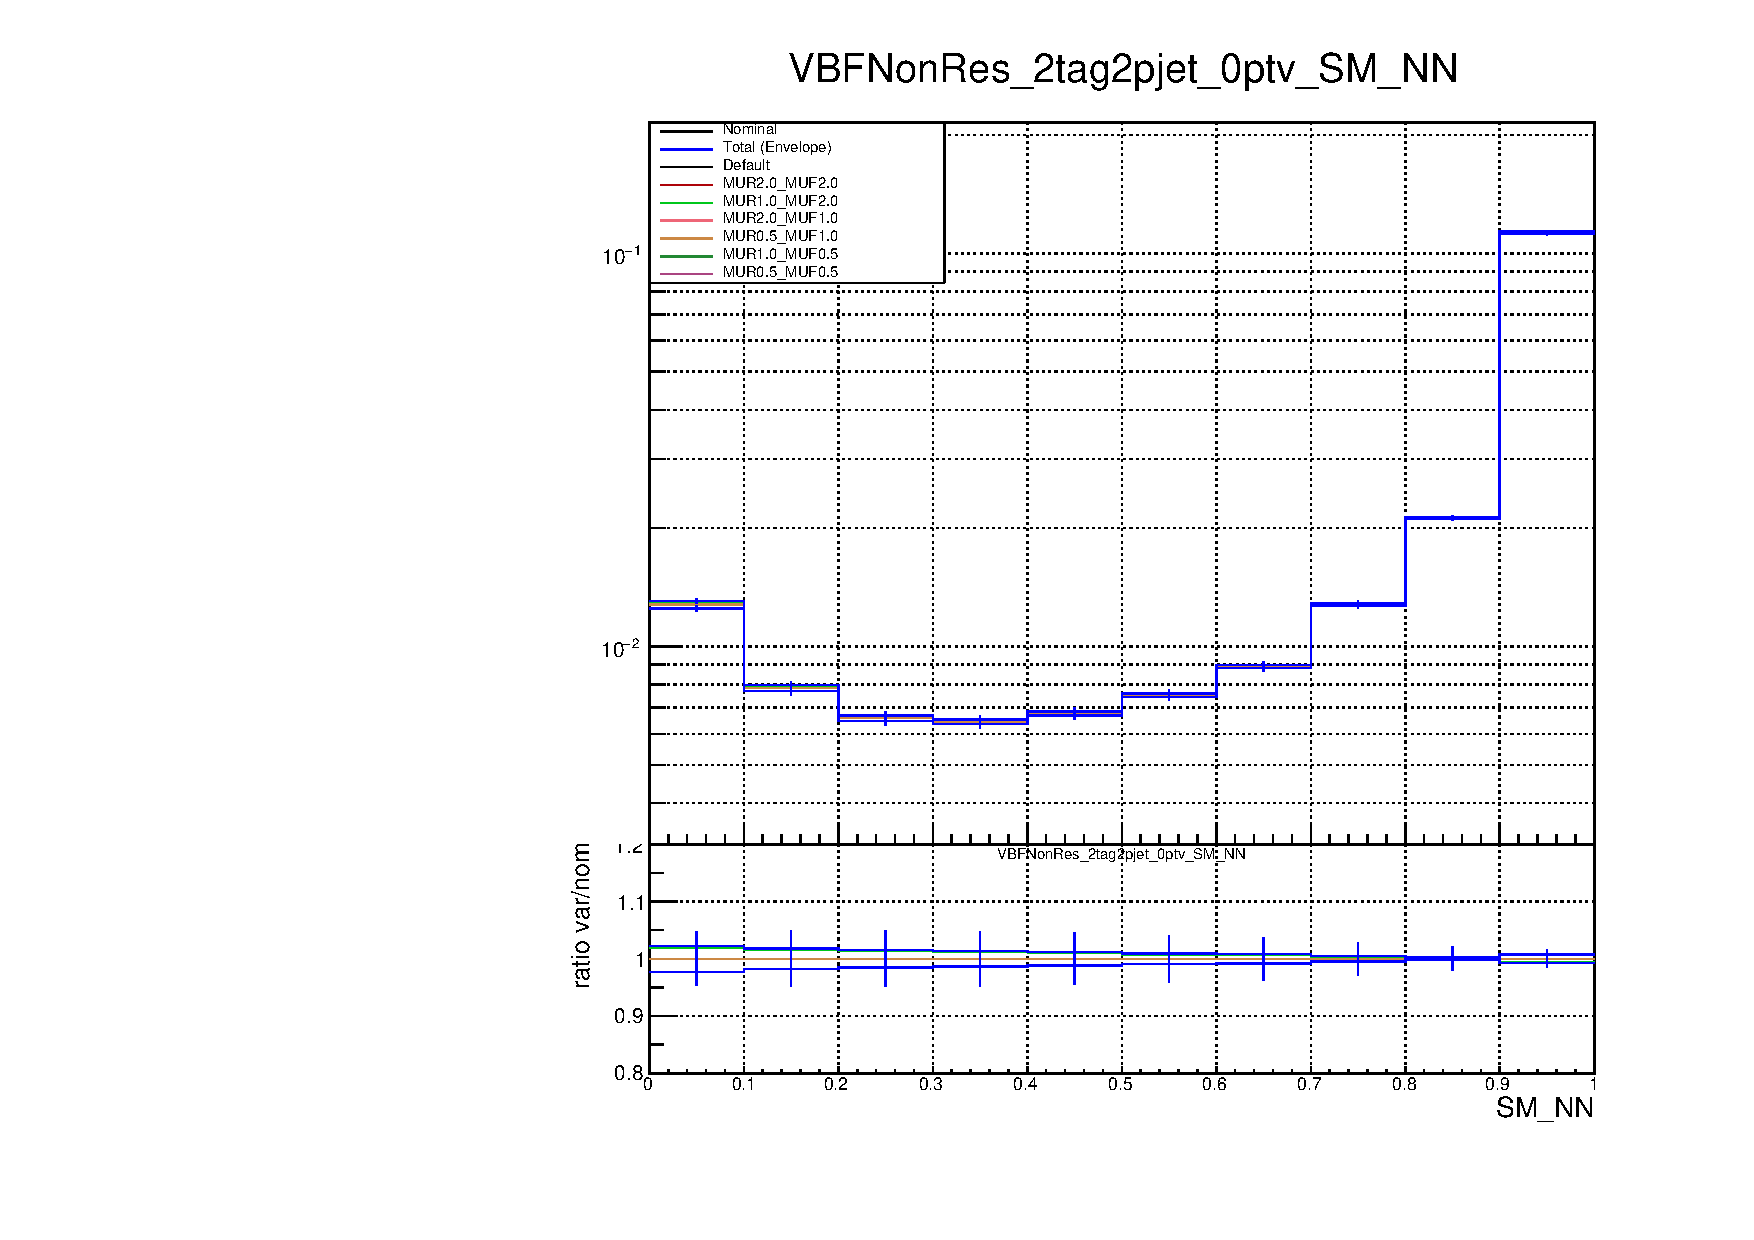
\includegraphics[width=0.5\textwidth]{figures/systs/lephad_vbf/VBFNonRes_Scale_SM_NN_SLT.pdf}}
  \subfloat[]{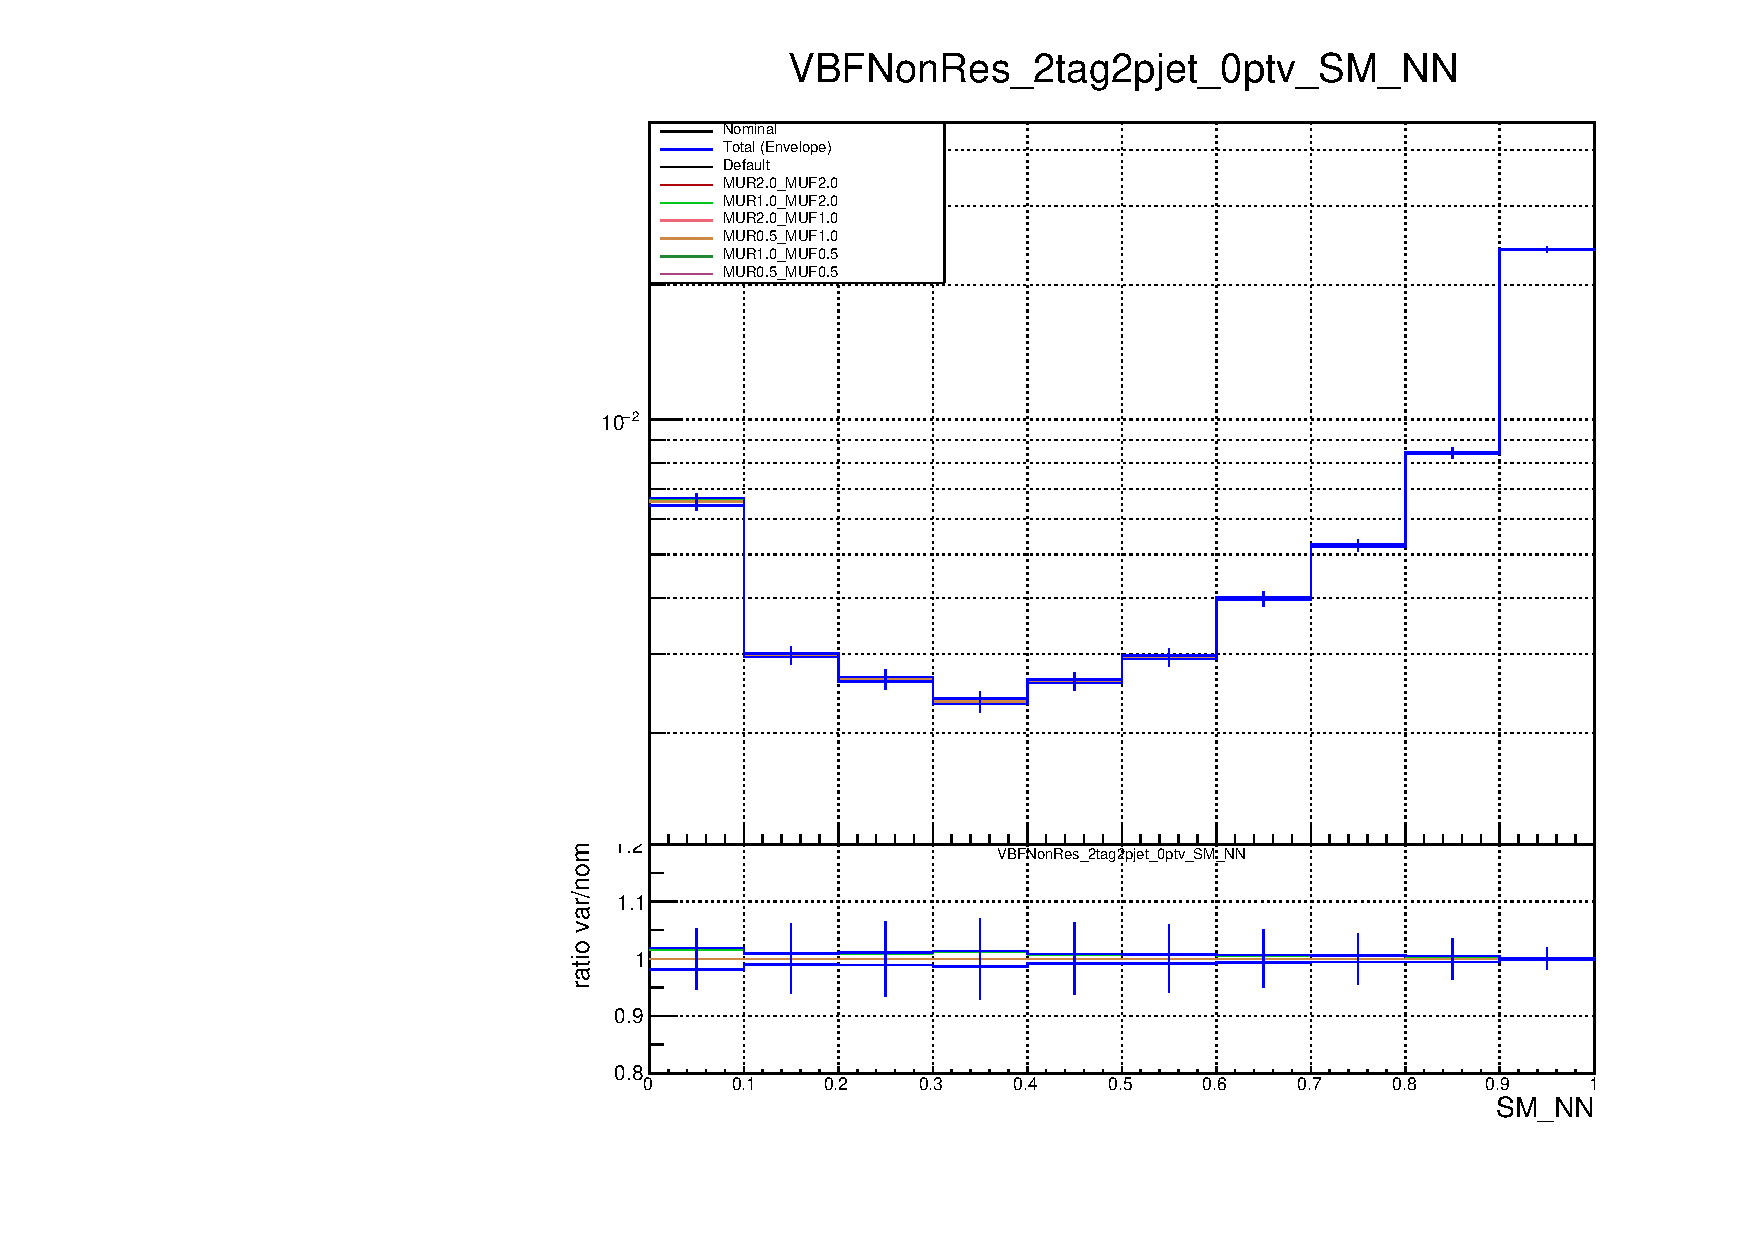
\includegraphics[width=0.5\textwidth]{figures/systs/lephad_vbf/VBFNonRes_Scale_SM_NN_LTT.pdf}}\\
  \subfloat[]{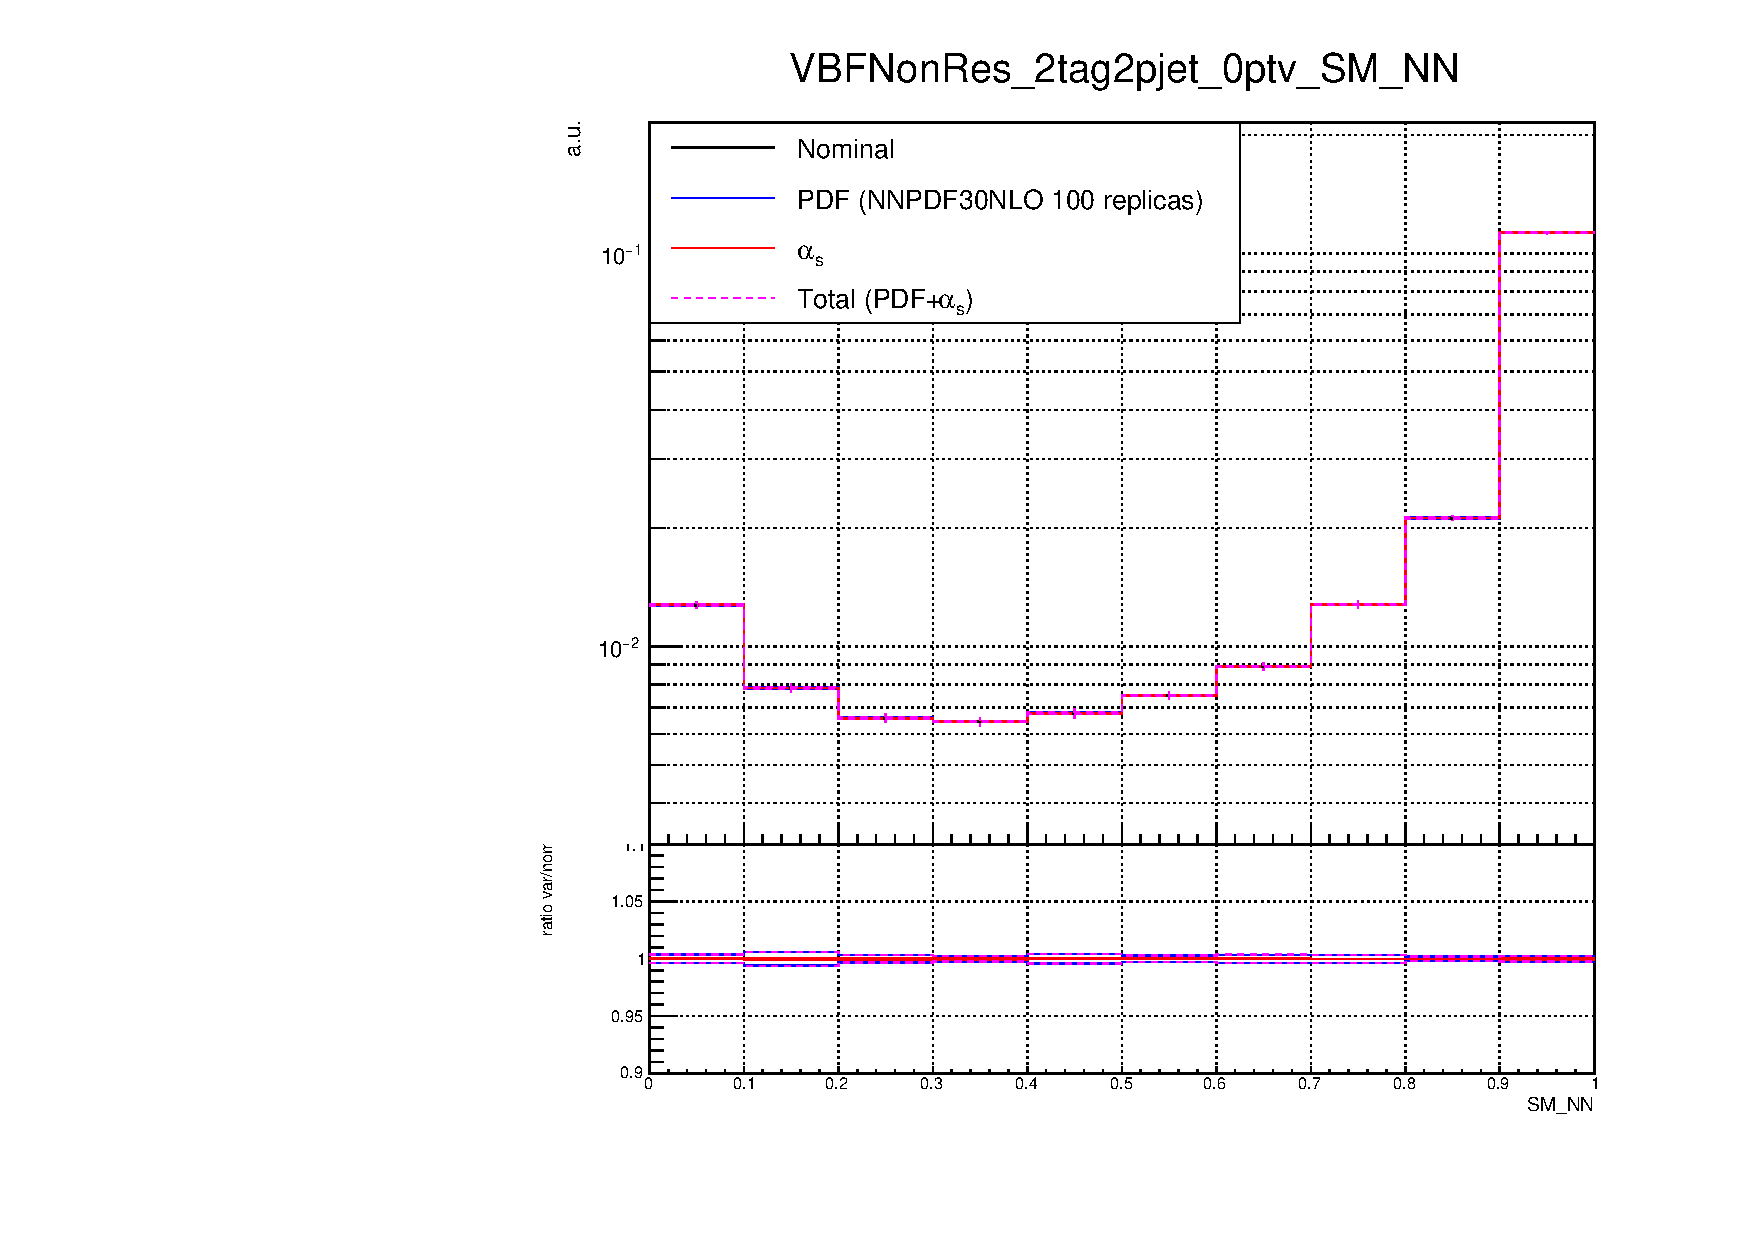
\includegraphics[width=0.5\textwidth]{figures/systs/lephad_vbf/VBFNonRes_PDF_SM_NN_SLT.pdf}}	
  \subfloat[]{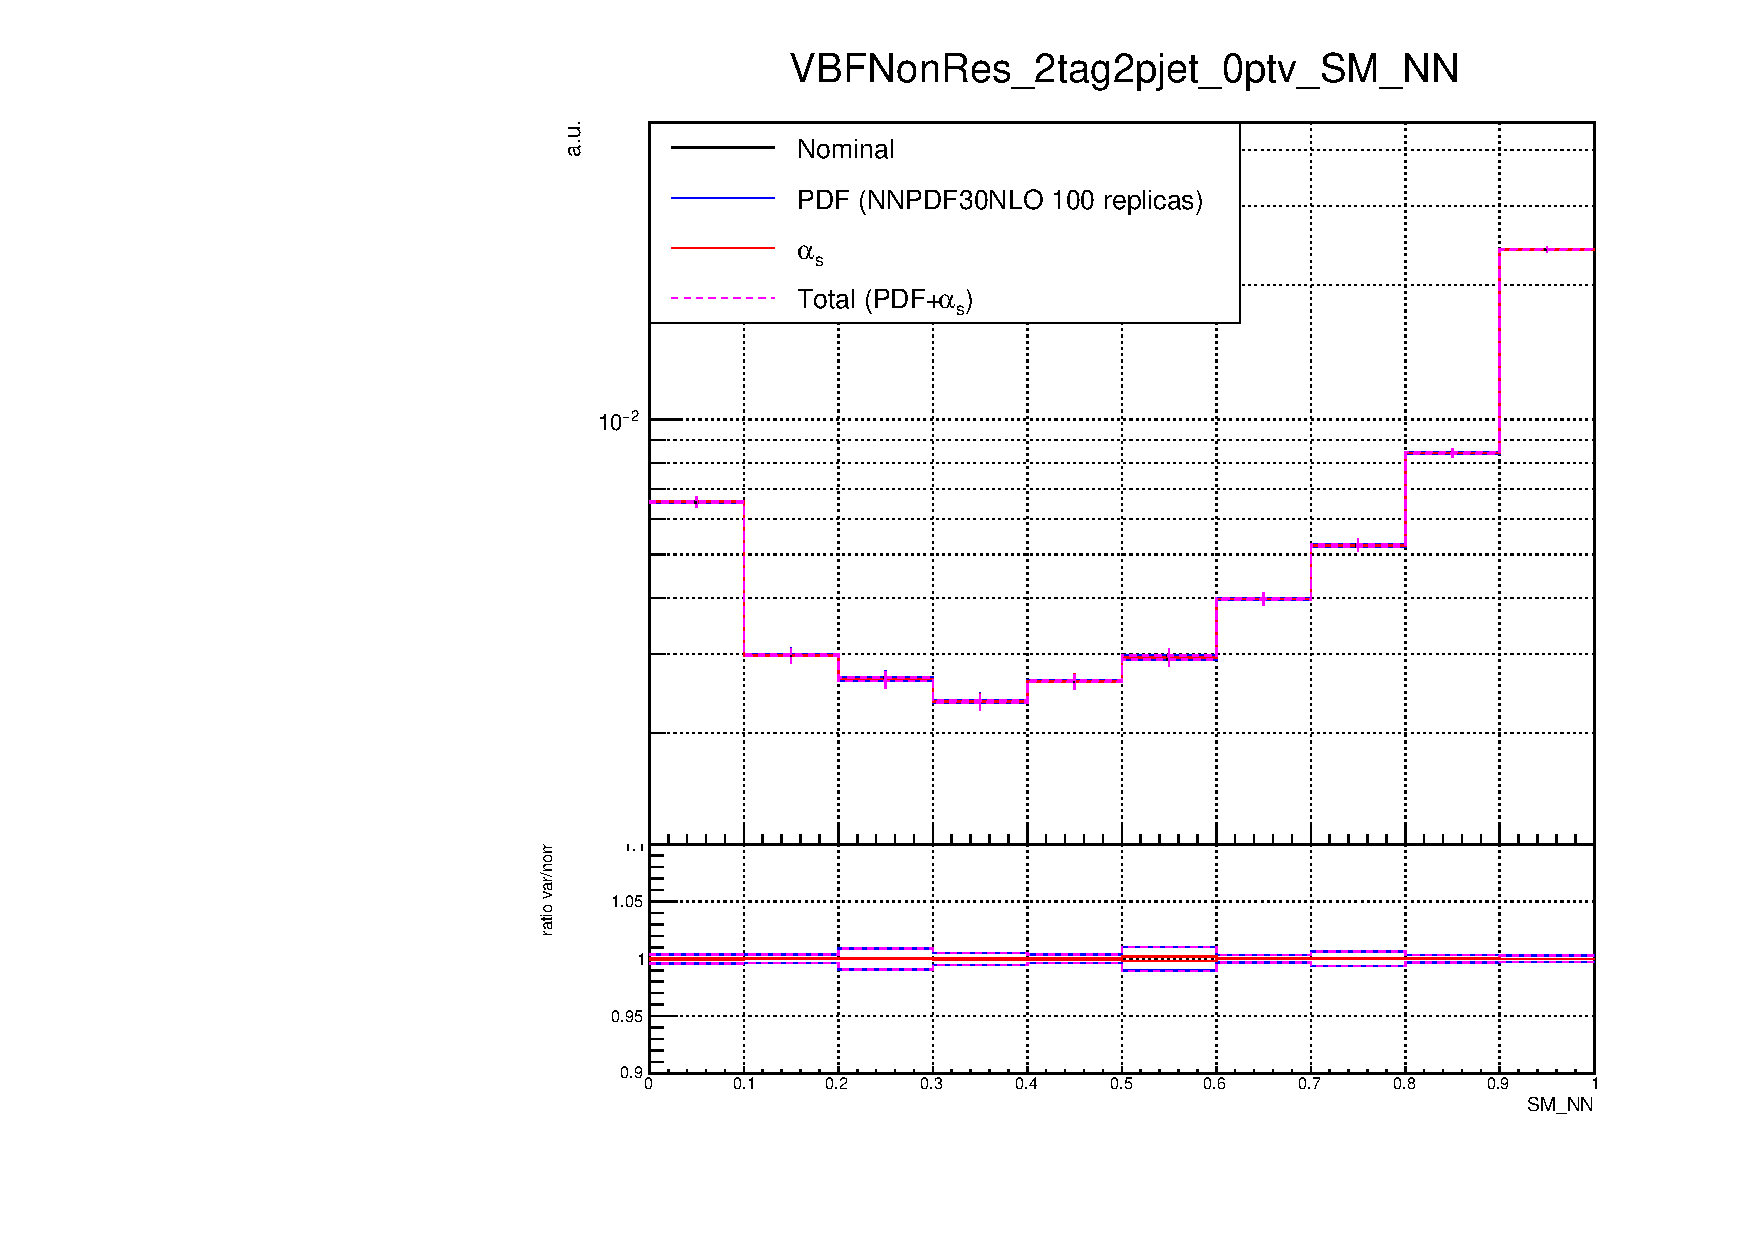
\includegraphics[width=0.5\textwidth]{figures/systs/lephad_vbf/VBFNonRes_PDF_SM_NN_LTT.pdf}}
  \caption{Impact of the 7-point scale variations on the final
    discriminant (SMNN) in the SR of the \lephad SLT channel (a) in the LTT channel (b), 
    and the PDF+\alphas uncertainties in the SLT channel (c), in the LTT channel (d).}
  \label{fig:lephad_vbf_scale_pdf}
\end{figure}


\begin{figure}[htbp]
  \centering

  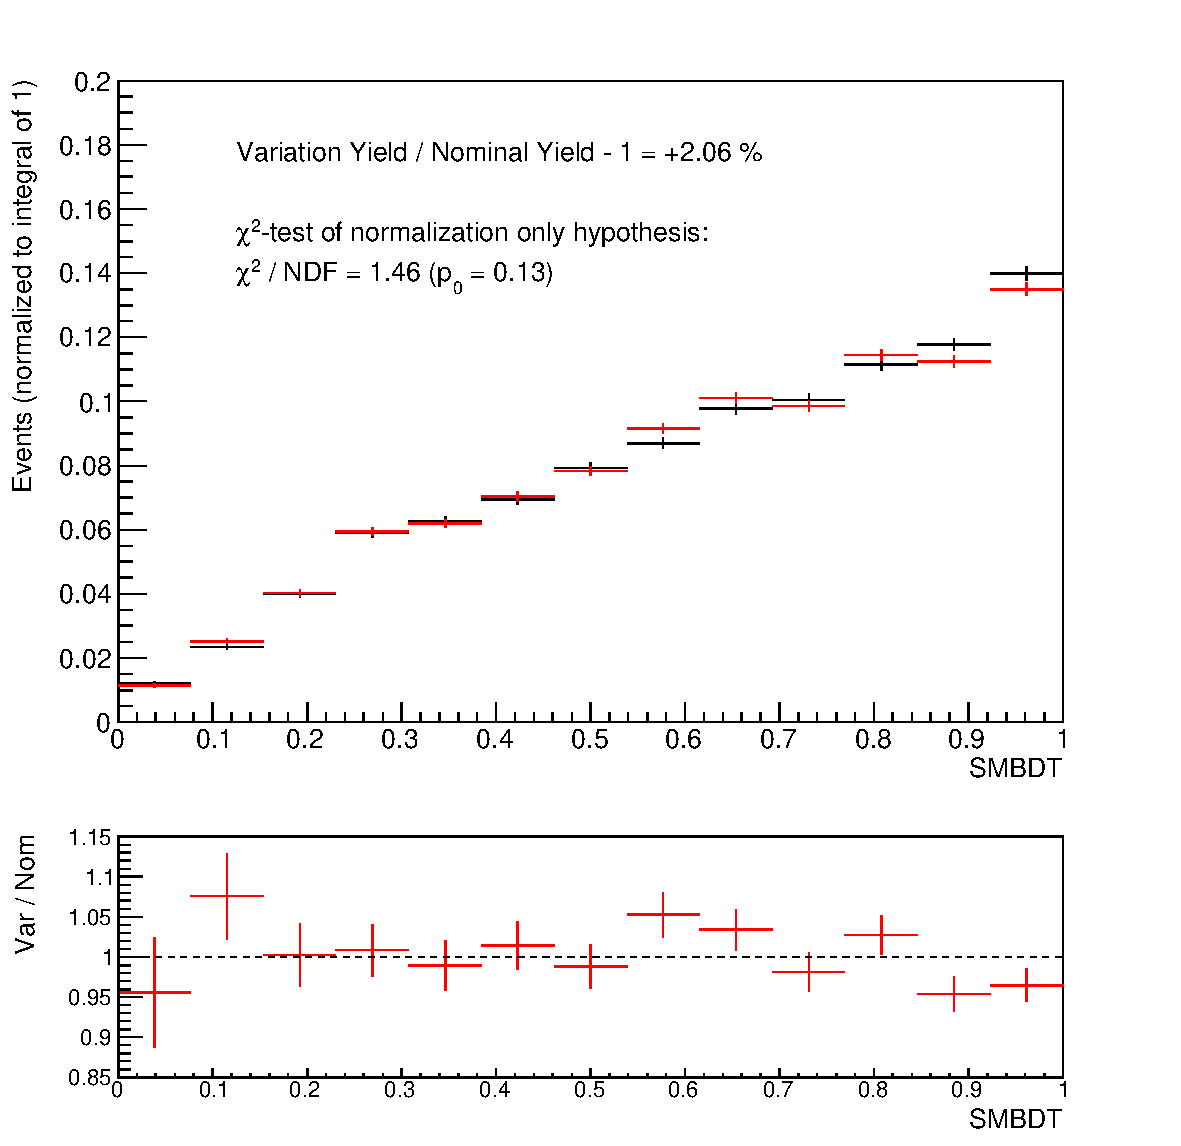
\includegraphics[width=0.5\textwidth]{figures/systs/hadhad_vbf/ps}

  \caption{Comparison of the alternative parton shower (Herwig7, red)
    with the nominal VBF signal sample (Pythia8, black) in the SR of
    the \hadhad-channel. To compare the shape-impact of this source of
    uncertainty, both histograms are normalised to the same integral
    before comparison. The uncertainty assigned due to PS algorithm is
    rounded up to 3 \% so that it also covers the deviations seen in
    the most significant SMBDT bins (note the difference in these bins
    before removing the normalisation from both histograms is
    $\approx \SI{3}{\percent}$) since this is where the analysis is
    most sensitive to the VBF HH contribution.}
\label{fig:vbf_uncertainties_ps}
\end{figure}

\begin{figure}[htbp]
  \centering

  \subfloat[]{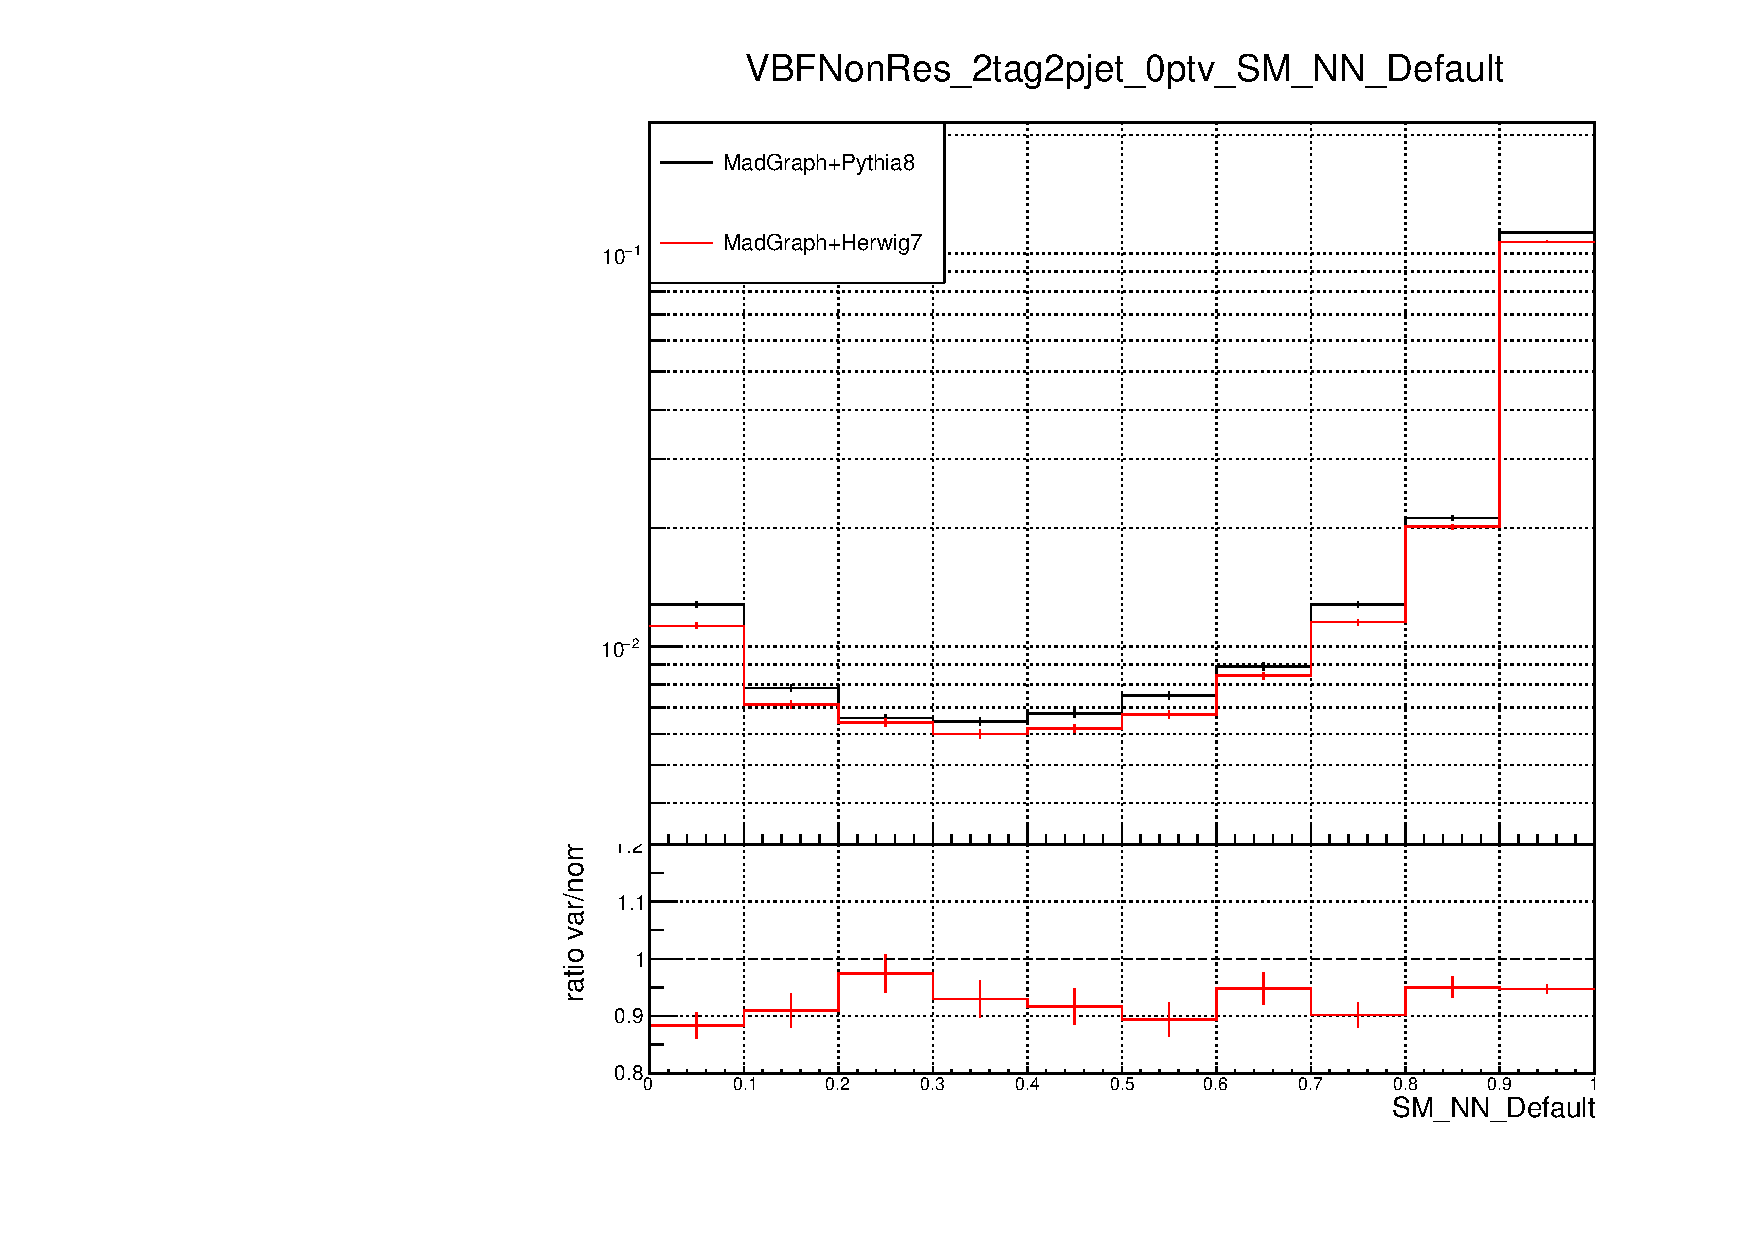
\includegraphics[width=0.5\textwidth]{figures/systs/lephad_vbf/VBFNonRes_PS_SM_NN_SLT.pdf}}
  \subfloat[]{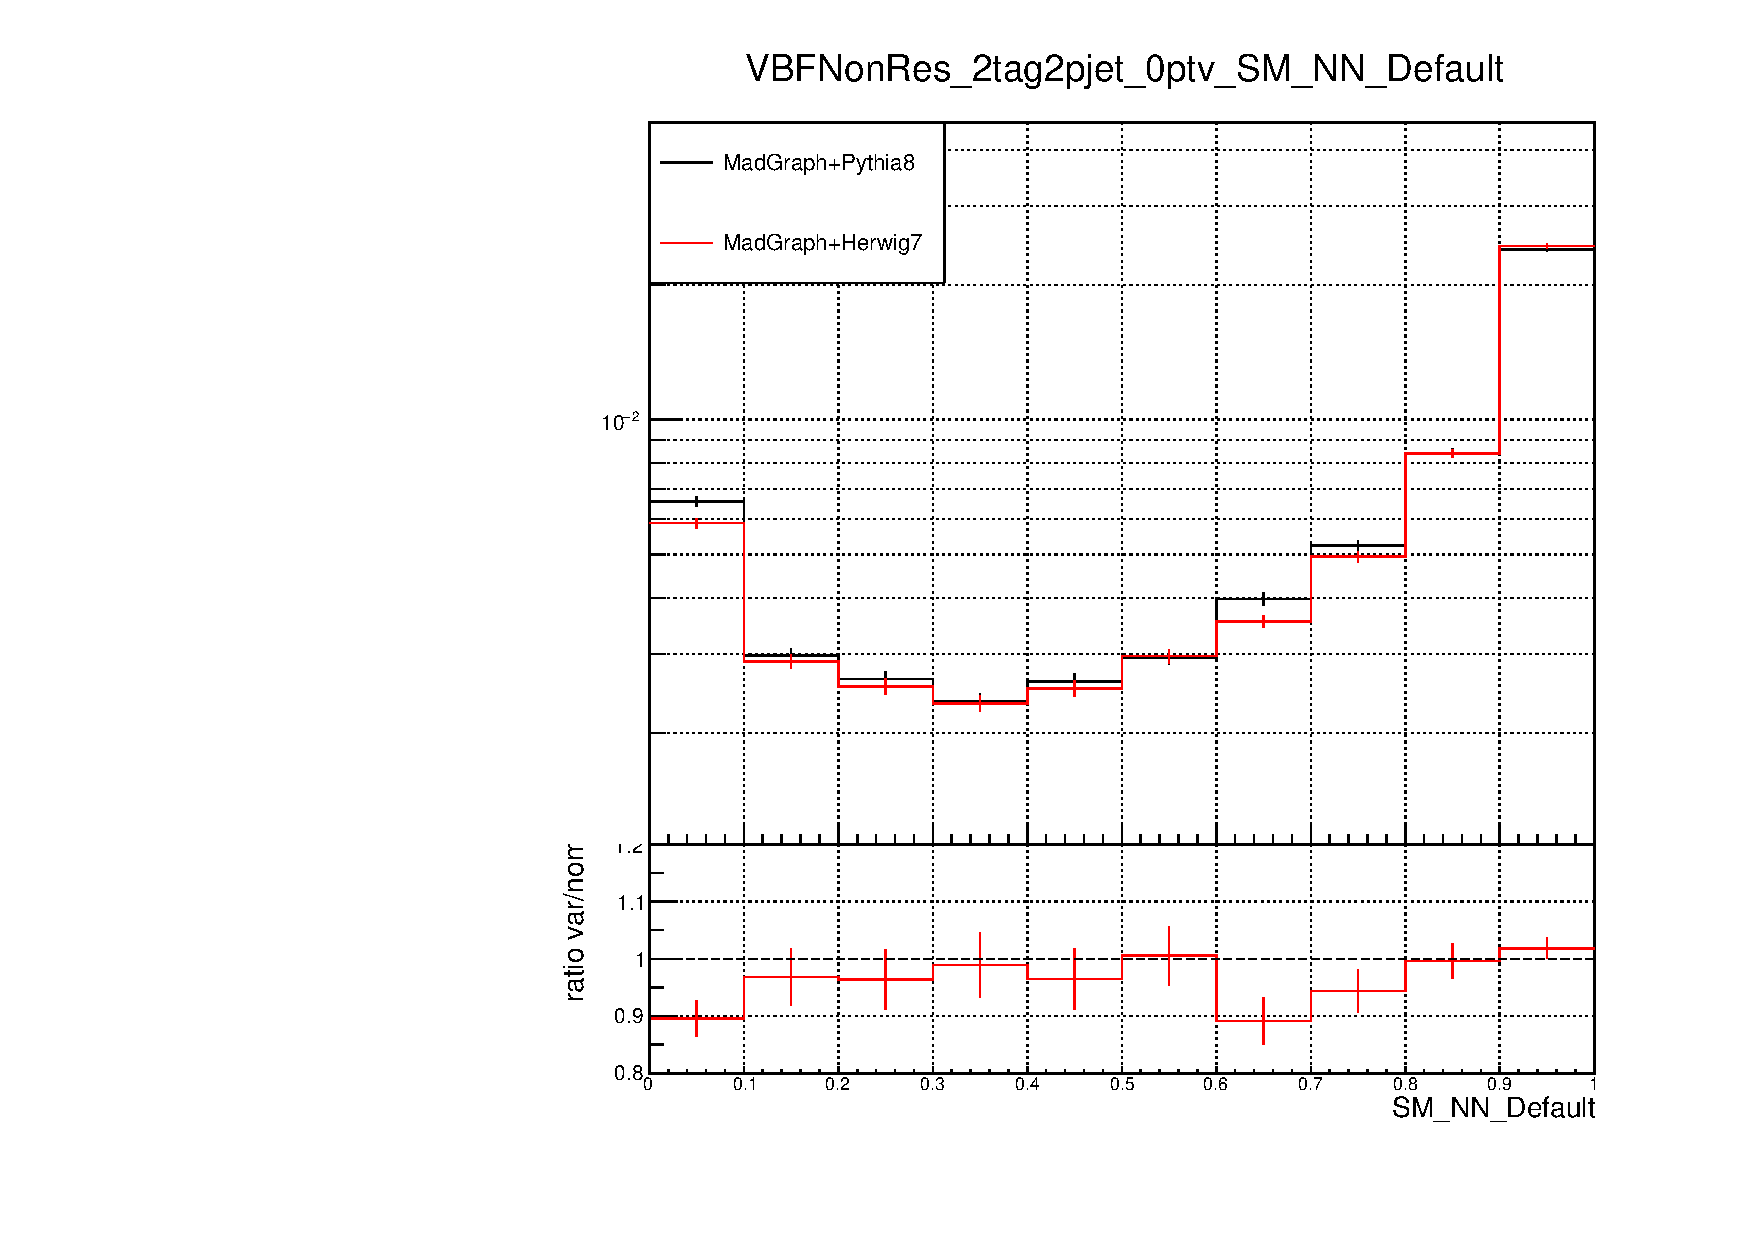
\includegraphics[width=0.5\textwidth]{figures/systs/lephad_vbf/VBFNonRes_PS_SM_NN_LTT.pdf}}

  \caption{Comparison of the alternative parton shower (Herwig7, red)
    with the nominal VBF signal sample (Pythia8, black) in the SR of
    the \lephad SLT channel (a), in the LTT channel (b). The uncertainty assigned due to PS algorithm is
    6.3\% (2.1\%) for the SLT (LTT) channel, which covers the deviations seen in
    the most significant SMNN bins.}
\label{fig:lephad_vbf_ps}
\end{figure}



\begin{table}
\centering
\small
\begin{tabular}{|c|c|c|c|c|}
\hline
Process & HadHad & LepHad SLT & LepHad LTT & Description\\
\hline
SM  & 3\,\% & 6.3\,\% & 2.1\,\% & Parton Shower\\
SM & 1\,\% &  0.15\,\% &  0.23\,\% & PDF+$\alpha_s$ from NNPDF30NLO errorset\\
SM & $\approx 0\,\%$ &  0.86\,\% &  0.63\,\% & Scales \\
\hline
\end{tabular}
\caption{List and relative size of VBF HH non-resonant signal acceptance uncertainties in the individual signal regions.}
\label{sec:systs:tab:systematics_HHNonResSignalVBF_AcceptanceNumbers}
\end{table}

Cross section uncertainties are also included, with values from \href{https://twiki.cern.ch/twiki/bin/view/LHCPhysics/LHCHWGHH?redirectedfrom=LHCPhysics.LHCHXSWGHH#Latest_recommendations_for_gluon}{\underline{LHCHHWG}} recommendations, shown in Table~\ref{sec:systs:tab:systematics_HHNonResSignalVBF_XSecNumbers}.

\begin{table}
\centering
\small
\begin{tabular}{|c|c|}
\hline
Source & Uncertainty\\
\hline
Scale & -0.0004, +0.0003\\
PDF + $\alpha_s$ & 0.021\\
\hline
\end{tabular}
\caption{List and relative size of VBF HH non-resonant SM signal cross section uncertainties.}
\label{sec:systs:tab:systematics_HHNonResSignalVBF_XSecNumbers}
\end{table}


